\documentclass[sigconf,anonymous,review]{acmart}
\usepackage{popets}

% --- Fonts ---
% acmart wants libertine + zi4 (inconsolata) + newtxmath, but silently falls back
% to Computer Modern if any of the three is missing.  The CM fallback pulls in the
% TS1 fonts (tcrm*), which have no Type1 version in BasicTeX, and microtype's font
% expansion then aborts with "auto expansion is only possible with scalable fonts".
% Loading the ACM text/math fonts ourselves avoids that and matches ACM typography.
% (If you install inconsolata -- see below -- these four lines become redundant and
%  can be deleted so that zi4 supplies the monospace font.)
\usepackage[T1]{fontenc}
\usepackage[tt=false,type1=true]{libertine}
\usepackage[libertine]{newtxmath}
\renewcommand{\ttdefault}{lmtt}

% Copyright
\setcopyright{popets}
\copyrightyear{2027}

% Issue info (filled at camera-ready)
\acmYear{2027}
\acmVolume{2027}
\acmNumber{X}
\acmDOI{XXXXXXX.XXXXXXX}
\acmISBN{}
\acmConference{Proceedings on Privacy Enhancing Technologies}
\settopmatter{printacmref=false,printccs=false,printfolios=true}

% --- Packages for our content (acmart already provides amsmath, booktabs, graphicx,
%     hyperref, xcolor, natbib; only add what is missing) ---
\let\Bbbk\relax % newtxmath already defines \Bbbk; let amssymb redeclare it
\usepackage{amssymb,amsfonts}
\usepackage{bm}
\usepackage{algorithm}
\usepackage{algpseudocode}

% --- Draft-only helper (remove once all TODOs are resolved) ---
\newcommand{\TODO}[1]{\textcolor{red}{[TODO: #1]}}

\begin{document}

\title[Grid-Guided Model Extraction]{Grid-Guided Model Extraction:
Stealing Interpretable Classifiers Without the Explanation}

% Anonymous submission: the [anonymous] class option suppresses author identity.
\author{Anonymous Author(s)}
\affiliation{%
  \institution{Submitted for double-blind review}
  \country{}}
\email{}
\renewcommand{\shortauthors}{Anonymous}

\begin{abstract}
Explanation-guided model extraction attacks steal a black-box classifier faster when the service
returns a post-hoc \emph{explanation} alongside each prediction, and the gain is normally credited to
the explanation's model-specific content. We show that credit is misplaced, and we turn the finding
into an attack. Decomposing what an explanation can contribute to query synthesis into a
feature-\emph{attribution} channel (which features matter) and a decision-\emph{threshold} channel
(where along a feature the prediction changes), we find through controlled ablations---each evaluated
over ten independent target instantiations---that attribution, the genuinely model-specific part,
confers no systematic advantage for either explainer: \textsc{Shap}-ranked feature choice is
indistinguishable from random, and \textsc{Lime}'s ranking is centred on zero with significant effects
in both directions. The channel that does help is the decision threshold exposed by \textsc{Lime}'s
discretization, worth up to $41$ fidelity points---but that threshold is a quantile of the background
distribution, not a property of the model, and refitting the discretizer on data the adversary already
holds reproduces the gain in full. We therefore build \emph{grid-guided extraction}: an attack that
never queries an explanation endpoint, snapping queries to a discretization grid it computes from its
own auxiliary sample and spending the saved budget on diverse generation and boundary search. On
tabular targets with continuous features it beats the explanation-guided attack it derives from by
$5.3$ fidelity points at an identical query budget (six significant gains against one loss over
sixteen target/dataset pairs) while issuing zero explanation calls, so it applies unchanged to
prediction-only services. On purely categorical targets it does not: with no continuous axis to
discretize there are no bin edges to exploit, and there the explanation retains real value. What a published explanation contributes to extraction is query-placement
convenience, not disclosure; the adversary is better off supplying that convenience itself.
\end{abstract}

\keywords{model extraction, model stealing, explainable AI, SHAP, LIME,
machine-learning-as-a-service, privacy}

\maketitle

% =======================================================================
\section{Introduction}
Machine-learning services increasingly return a post-hoc \emph{explanation} alongside each
prediction. Cloud providers ship attribution APIs as standard tooling, and regulatory pressure---the
GDPR's provisions on automated decision-making, and more recently the EU AI Act's transparency
obligations---pushes deployments further in that direction. The premise is that a prediction
accompanied by a reason is more accountable than a prediction alone.

That premise has a security cost, because an explanation is additional output computed from the very
model an adversary would like to steal. Model extraction reconstructs a functional copy of a
black-box target from query access~\cite{tramer2016stealing,jagielski2020high}, and the resulting
surrogate is not merely an intellectual-property loss: it is a platform for further attacks, since a
functionally equivalent copy enables membership inference at a fraction of the direct query
cost~\cite{oksuz2026lomime,ezzeddine2026membership}. If explanations make extraction materially
cheaper, then transparency and privacy are in direct tension, and providers face a genuine trade-off.

Explanation-guided extraction attacks report exactly that: querying with explanations attached yields
higher-fidelity surrogates for fewer queries~\cite{oksuz2024autolycus,milli2019model,aivodji2020model}.
These results establish \emph{that} explanations help, and are typically reported end-to-end: the
attack is run with the explanation and compared against a baseline without it. The gain is then
naturally credited to the explanation's model-specific content---which features the model relies on
locally, or, for gradient explanations, the local geometry of the decision boundary. An end-to-end
comparison, however, cannot separate that content from the other things an explanation supplies, such
as a convenient set of coordinates at which to place the next query. Which of these is responsible
matters practically, because it determines whether the risk attaches to explanations as such, to
particular explanation methods, or to something an adversary could obtain anyway.

\paragraph{This paper.} We decompose what an explanation can contribute to an attacker's query
synthesis into two channels: an \emph{attribution} channel (\emph{which} features are locally
influential) and a \emph{threshold} channel (\emph{where} along a feature the prediction changes).
The distinction is not merely conceptual---it separates the two dominant explanation families.
\textsc{Shap} reports signed magnitudes and exposes only the first; \textsc{Lime}, which discretizes
continuous features before fitting its local surrogate, exposes both, since its bin edges are
candidate decision thresholds. We ablate each channel independently inside a state-of-the-art
explanation-guided attack, holding the traversal, the seeds, and the random state fixed, and evaluate
every comparison over ten independent target instantiations.

The attribution channel---the part of an explanation that is genuinely model-specific---confers no
systematic advantage for either explainer: replacing the explanation's feature ranking with a random
choice leaves fidelity centred on zero, with significant effects in \emph{both} directions depending
on the target. The one channel that reliably helps is \textsc{Lime}'s discretization threshold, which
is worth up to $41$ fidelity points. But that threshold is a quantile of the background data, not a
property of the model: when we refit the discretizer on data the adversary already holds, the gain is
reproduced in full, and the advantage of the target's own discretizer is statistically
indistinguishable from zero.

\paragraph{From diagnosis to attack.} These findings are not merely negative results about
explanations; read constructively, they specify a better adversary. If attribution is inert and the
useful threshold is self-computable, then the explanation endpoint is not worth querying: an attacker
should compute the grid itself and spend its budget on placing queries where the surrogate is actually
uncertain. We build that attack---\emph{grid-guided extraction}---by combining a self-computed
discretization with diverse query generation and boundary search
(\S\ref{sec:method}). It never calls an explanation endpoint. On targets with continuous features it
beats the explanation-guided baseline it derives from by $5.3$ fidelity points at an identical query
budget, and because it needs no explanation it applies unchanged to prediction-only services, where an
explanation-guided attack cannot be mounted at all. On purely categorical targets the mechanism has
nothing to bite on and the baseline wins; we report that boundary rather than tuning around it. What a published explanation contributes to extraction is
therefore \emph{query-placement convenience}, not disclosure---and an adversary is better off supplying
that convenience itself.

\paragraph{Contributions.}
\begin{itemize}
  \item \textbf{Grid-guided extraction}, an attack that exceeds explanation-guided extraction on
  continuous-feature targets ($+5.3$pp, six significant gains against one loss) without querying an
  explanation endpoint, by pairing a self-computed discretization grid with diverse query generation
  and boundary search. Because it makes zero explanation calls it runs against prediction-only
  services, which the attack it derives from cannot (\S\ref{sec:method}, \S\ref{subsec:ladder}).
  \item An evaluation ladder that separates \emph{what an adversary needs} from \emph{what a service
  gives it}: four adversaries differing only in whether they hold the target's explanation, their own
  grid, or neither, run within the same framework, budget, seeds and evaluation set
  (\S\ref{subsec:ladder}).
  \item A two-channel decomposition of explanation leakage (attribution versus threshold) that makes
  ``what does an explanation leak'' an answerable empirical question, and a protocol for testing it
  that isolates each channel while holding the rest of the attack fixed (\S\ref{sec:problem},
  \S\ref{sec:analysis}).
  \item Evidence that the attribution channel confers no systematic extraction advantage---for
  \textsc{Shap} and for \textsc{Lime} alike---and that where explanation-guided selection does have a
  significant effect, its \emph{sign} is a property of the target rather than of the explanation
  (\S\ref{subsec:e2}).
  \item Evidence that the threshold channel, which does help substantially, is
  \emph{self-computable}: an adversary holding a modest auxiliary sample reconstructs an equivalent
  discretization with no measurable loss, so the channel is not a disclosure by the service
  (\S\ref{subsec:e3}, \S\ref{subsec:e5}).
\end{itemize}

\paragraph{Scope.} Our conclusions are bounded in ways worth stating up front. We study one family of
explanation-guided attack---traversal-based extraction against interpretable
classifiers~\cite{oksuz2024autolycus}---on tabular data, with two explainers in their default
configurations. A differently designed attack, or a discretizer that depends on labels rather than on
the marginal distribution, could plausibly extract more from the same explanations. We therefore claim
that post-hoc explanations leak considerably less than the literature assumes \emph{in this setting},
not that they are harmless in general.

% =======================================================================
\section{Background and Related Work}
\label{sec:background}

\subsection{Model Extraction and Post-hoc Explanations}
\label{subsec:prelim}

Model extraction attacks reconstruct a functional copy $\hat{f}$ of a black-box
target $f$ from query access alone, with success measured by \emph{prediction
agreement} between $\hat{f}$ and $f$ on held-out data (formalised in
\S\ref{sec:problem}). When the target is deployed as an explainable service, each
query returns not only a label but a post-hoc \emph{explanation}, which may reveal
additional structure about $f$. Two dominant explanation families expose
fundamentally different information:

\begin{itemize}
  \item \textbf{Attribution methods (SHAP).} SHAP~\cite{lundberg2017shap} assigns
  each feature a signed magnitude $\phi_i(x)$---its Shapley marginal contribution
  to the prediction at $x$. This is a statement of \emph{how much} each feature
  matters locally; it carries no explicit information about \emph{where} along a
  feature axis the decision changes.
  \item \textbf{Local surrogate methods (LIME).} LIME fits an interpretable model
  to a \emph{discretized} neighbourhood of $x$: continuous features are binned, and
  the returned coefficients are attached to $(\text{feature}, \text{bin})$ pairs.
  LIME therefore reveals both an influential feature \emph{and} the bin edge---a
  \emph{threshold}---that separates neighbouring regions.
\end{itemize}

This distinction between \emph{magnitude-only} and \emph{threshold-bearing}
explanations is central to our analysis: as we show, it is the threshold, not the
attribution magnitude, that an extraction attacker can exploit
(\S\ref{sec:problem}, \S\ref{sec:analysis}).

\subsection{Related Work}
\label{subsec:related}

\paragraph{Model Extraction Attacks}
Model extraction attacks aim to reconstruct a functional copy of a black-box target model through strategic querying~\cite{tramer2016stealing}.
Early work by Tram\`er~et~al.~\cite{tramer2016stealing} demonstrated that
simple equation-solving over prediction outputs suffices for linear models.
Subsequent methods scaled to neural networks: Knockoff Nets~\cite{orekondy2019knockoff}
trains a surrogate on outputs obtained by querying with a knock-off dataset,
while Jagielski~et~al.~\cite{jagielski2020high} show that high-fidelity extraction
of deep networks is possible given sufficient queries.
A parallel line of work~\cite{papernot2017practical,correia2018copycat} frames
model extraction as knowledge distillation, transferring decision boundaries
through synthetic queries.
Marich~\cite{karmakar2023marich} formalises the problem as \emph{distributional equivalence}
and proposes an active sampling strategy that maximises information gain per query.
In contrast, our method requires only a small per-class seed set rather than a large
public transfer set, and synthesises informative queries from that seed.

\paragraph{Explanation-Guided Extraction.}
The observation that post-hoc explanations leak structural information about the
target model motivates a distinct attack family.
Milli~et~al.~\cite{milli2019model} first demonstrated that gradient-based explanations
suffice to reconstruct linear models exactly.
Autolycus~\cite{oksuz2024autolycus} extended this to classical ML classifiers
(decision trees, logistic regression, naive Bayes, and $k$-NN) by using LIME and SHAP
explanations as traversal guides: the attacker perturbs seed samples along the
directions of highest feature attribution, progressively labelling a synthetic dataset
to train a surrogate. Yan~et~al.~\cite{yan2023explanationleaks} (XaMEA) similarly
exploit the spatial information contained in explanations in a model-agnostic manner.
A common assumption, implicit in these attacks, is that the explanation's
\emph{attribution ranking} is what drives the extraction gain.
Through controlled ablations we revisit this assumption and find it does \emph{not}
hold: the gain stems primarily from boundary-directed query synthesis---boundary
search and diverse sampling---while the choice of features by attribution
contributes little beyond a random choice. The explanation supplies additional signal
only when it exposes a decision \emph{threshold}: LIME's discretization surfaces such
thresholds directly, whereas SHAP's magnitude attribution does not, so a SHAP-guided
attacker must \emph{search} for the boundary and gains little over the sampling
procedure itself. This reframes explanation leakage as a matter of decision
\emph{thresholds} rather than boundary \emph{geometry}.

\paragraph{Counterfactual-Based Extraction.}
A growing body of work exploits counterfactual explanations (CFs) rather than
attribution scores.
A\"ivodji~et~al.~\cite{aivodji2020model} first showed that CFs leak enough
boundary information to build high-fidelity surrogates, and DualCF~\cite{wang2022dualcf}
improved query efficiency by training on CF/counter-CF \emph{pairs} that
straddle the decision boundary.
Khouna~et~al.~\cite{khouna2025tra} propose the Tree Reconstruction Attack (TRA),
which uses a \emph{restricted} CF oracle to perform axis-aligned binary search,
achieving exact functional reconstruction of decision trees and random forests.
Although theoretically elegant, TRA requires an oracle that returns the
\emph{nearest} counterfactual confined to a specific hyper-rectangle---an assumption
rarely satisfied by deployed XAI APIs.
Concurrently, \citet{otto2026linear} derive query complexity bounds for extracting
linear classifiers under factual and counterfactual query regimes.
Our work connects these lines: rather than a bespoke CF oracle, we obtain boundary
thresholds from the explanation itself---directly from LIME's discretization, or by
SHAP-directed single-axis bisection---without requiring restricted oracle access.
Consistent with our central finding, it is this threshold signal, not the attribution
magnitude, that constitutes the exploitable channel.

\paragraph{Privacy Implications of Explanations.}
Recent work highlights the security cost of XAI transparency.
\citet{ezzeddine2026membership} show that counterfactual explanations amplify
membership inference attacks (MIAs) in MLaaS settings, characterising a
fundamental utility--privacy trade-off.
LoMime~\cite{oksuz2026lomime}---from the authors of Autolycus---uses surrogate model
extraction as a stepping stone for label-only MIA, demonstrating that functionally
equivalent surrogates enable downstream privacy attacks with far fewer queries than
direct methods; our extraction fidelity thus serves as an upstream component for such
attacks.
Surveys of privacy-preserving explanation~\cite{nguyen2024survey} catalogue
countermeasures. Localising the effect to a specific channel (the discretization
threshold) lets us ask what such a countermeasure would have to accomplish; we find
that obfuscating that channel is unlikely to suffice, since the adversary can
reconstruct an equivalent grid from its own data (\S\ref{subsec:e5}).

% =======================================================================
\section{Problem Formulation}
\label{sec:problem}

\paragraph{Setting.}
Let $f : \mathcal{X} \to \mathcal{Y}$ be a black-box target classifier, with
$\mathcal{X} \subseteq \mathbb{R}^d$ and $\mathcal{Y} = \{0, \ldots, C{-}1\}$.
The attacker knows neither $f$'s architecture nor its training data, and interacts
with $f$ only through an \emph{explanation-augmented prediction API}.
Each query $x \in \mathcal{X}$ returns (i) the predicted label $f(x)$ and the
class-probability vector $\hat{p}(x) \in \Delta^{C}$, and (ii) a post-hoc
explanation $e(x)$ produced by a fixed explainer
$\mathcal{E} \in \{\textsc{Shap}, \textsc{Lime}\}$.
Every call counts against a total query budget $Q$.
The attacker additionally holds a small per-class \emph{seed set}
$\mathcal{D}_{0} = \{(x_i, y_i)\}$ with $n$ examples per class (following the respective
Autolycus conventions, $n{=}1$ for \textsc{Lime} and $n{=}5$ for \textsc{Shap}), drawn from a
public split that shares $\mathcal{X}$'s feature schema;
this is a handful of seeds, not a large public transfer set.

\paragraph{Explanation oracle.}
The two explainers expose structurally different information about $f$ near $x$:
\begin{itemize}
  \item \textbf{\textsc{Shap}}: $e(x) = \bm{\phi}(x) \in \mathbb{R}^{d}$, a vector of
  signed Shapley attributions in which $|\phi_i(x)|$ measures the local influence
  \emph{magnitude} of feature $i$~\cite{lundberg2017shap}. It reports \emph{how much}
  each feature matters, but not \emph{where} the decision changes along it.
  \item \textbf{\textsc{Lime}}: $e(x) = \{(i,\, [l_i, u_i],\, w_i)\}_{i \in S}$ over a
  selected feature subset $S$, where feature $i$ has local weight $w_i$ and lies in
  the discretization bin $[l_i, u_i]$. Beyond a magnitude, \textsc{Lime} therefore
  discloses a \emph{bin edge} which is an estimate of a coordinate at which $f$'s output
  changes.
\end{itemize}

\paragraph{Objective.}
The attacker trains a surrogate $\hat{f} : \mathcal{X} \to \mathcal{Y}$ that is
\emph{functionally equivalent} to $f$, measured by prediction agreement:
\begin{equation}
    \mathrm{Sim}(\hat{f}, f) \;=\; \mathbb{E}_{x \sim P_{\mathcal{X}}}
    \bigl[\mathbf{1}(\hat{f}(x) = f(x))\bigr].
    \label{eq:sim}
\end{equation}
Here $P_{\mathcal{X}}$ is the (unknown) data distribution over $\mathcal{X}$,
estimated in practice by a held-out test set disjoint from the attacker's seed set
$\mathcal{D}_{0}$ and its queries.
The attack succeeds if $\mathrm{Sim}(\hat{f}, f)$ is high while the number of API
calls stays within $Q$. 
% We report $\mathrm{Sim}$ as a function of $Q$, so that \emph{query efficiency}---the operative cost for an extraction adversary---is explicit.

\paragraph{What does an explanation leak?}
The power of an extraction attack rests on \emph{query placement}: labelled queries
concentrated at the decision boundary and spread across diverse decision regions are far
more informative than interior or random queries, independent of any
explanation~\cite{pal2020activethief}. Our question is what a post-hoc explanation
\emph{adds} to this placement. We decompose the explanation's possible contribution into
two channels:
\begin{enumerate}
  \item \textbf{Attribution:} \emph{which} features are locally influential
  (a ranking by $|\phi_i|$ or $|w_i|$), available from both \textsc{Shap} and
  \textsc{Lime}.
  \item \textbf{Threshold:} \emph{where} along a feature axis the prediction
  changes, i.e.\ the coordinate of the decision boundary. \textsc{Lime}'s bin edge
  $\{l_i, u_i\}$ is a direct estimate; \textsc{Shap}'s magnitude carries no such
  location.
\end{enumerate}
Each channel admits a sharp null hypothesis, and our experiments resolve them in opposite directions:
the attribution channel is inert (\S\ref{subsec:e2}), while the threshold channel is the one that
operates (\S\ref{subsec:e3})---but is reproducible from the adversary's own data rather than disclosed
by the service (\S\ref{subsec:e5}). We treat that pair of findings as a design specification rather
than as a conclusion, and build the attack it implies (\S\ref{sec:method}, \S\ref{subsec:ladder}).

Neither channel is an attack in itself. The query-placement machinery of \S\ref{sec:method}---boundary
search and diverse generation---is a standard extraction technique that the explanation does not
disclose and that an attacker can run without any explanation at all. What an explanation can change is
only \emph{where} that machinery directs its queries: the attribution channel proposes which coordinate
to move along, and the threshold channel proposes how far to move it. Isolating these two inputs is
therefore the natural way to ask what the explanation itself contributes. Prior explanation-guided
attacks~\cite{oksuz2024autolycus,milli2019model} implicitly credit their gain to the
\emph{attribution} channel and, for gradient explanations, to recovering boundary \emph{geometry} (the
local normal). Our central hypotheses, examined
in \S\ref{sec:analysis} and \S\ref{sec:experiments}, are:
\begin{description}
  \item[\textbf{H1 (attribution is inert).}] Steering query placement by explanation
  importance does not improve fidelity over a random feature choice. The attack's gain
  comes from query placement itself, not from the attribution channel.
  \item[\textbf{H2 (the threshold is the operative channel).}] The only explanation-supplied
  signal that improves fidelity is the threshold channel. A threshold-bearing explainer
  (\textsc{Lime}) helps, whereas a magnitude-only explainer (\textsc{Shap}) does not,
  because---lacking a threshold---it must \emph{search} for the boundary.
  \item[\textbf{H3 (the threshold is not a disclosure).}] The threshold that helps is a
  statistic of the \emph{data distribution}---\textsc{Lime}'s default bin edges are quantiles
  of its background sample, independent of the model and of the labels---rather than a
  property of the target. An adversary holding a modest auxiliary sample can therefore
  reconstruct an equivalent grid, so the channel accelerates extraction without the service
  disclosing anything the adversary could not compute itself.
\end{description}
H1 and H2 together locate \emph{which} part of an explanation an attacker consumes; H3 asks
whether consuming it required the explanation at all. That last question is the organising
principle of this paper: leakage should be measured against what the adversary could obtain
unaided, not against nothing.

\paragraph{Threat model.}
We assume: (1)~black-box access only (no white-box gradients); (2)~the API returns
post-hoc explanations (\textsc{Shap} or \textsc{Lime}), as increasingly expected for
transparency (e.g.\ GDPR Article~22); (3)~the attacker knows the feature schema but
not the model family or hyperparameters; and (4)~the attacker holds a small auxiliary
sample $D_A$ drawn from the target's distribution, from which it draws $n{\le}5$ seeds per
class. Assumption~(4) is inherited from the attack we analyse~\cite{oksuz2024autolycus},
which allows $D_A$ to range ``from a rudimentary collection of samples to comprehensive
datasets''; it matters here because H3 turns on what the adversary can estimate from $D_A$
alone. This captures realistic MLaaS deployments in which a vendor exposes explanations for
regulatory compliance without revealing the underlying model.

% =======================================================================
\section{Method}
\label{sec:method}
This section describes a three-phase query-synthesis pipeline---diverse generation, boundary search,
and traversal---that we run in \emph{two configurations}. The distinction matters throughout the
paper, so we fix the names here.

\begin{description}
  \item[\textsc{grid-guided} (the attack we propose).] Every phase takes its coordinates from a
  discretization grid the adversary computes from its \emph{own} auxiliary sample, and features are
  chosen at random. No explanation endpoint is queried. This is the constructive consequence of the
  diagnosis in \S\ref{sec:analysis}---attribution is inert and the useful threshold is
  self-computable---and it is what the title claims and \S\ref{subsec:ladder} evaluates.
  \item[\textsc{explanation-matched} (a comparison configuration).] The same three phases, but with
  the target's \textsc{Lime} output supplying the feature ranking and the bin edges, exactly as
  Autolycus consumes it. This configuration exists to compare query \emph{placement} against the
  published baseline at equal information access (\S\ref{subsec:e4}, \S\ref{subsec:e1}); it is not the
  attack we advocate.
\end{description}

\noindent The second configuration also serves as a measurement instrument: it gives the explanation
channels every chance to be useful, so a null result cannot be dismissed as the artefact of a weak
adversary. Two properties make that role credible. First, the channel ablations of \S\ref{subsec:e2},
\S\ref{subsec:e3} and \S\ref{subsec:e5} all run on the \emph{base} Autolycus traversal, which contains
none of the machinery below, so those conclusions do not depend on our additions. Second, every phase
described here has an explanation-free implementation: Phase 1 uses no model output at all, and Phases
2 and 3 consume only bin edges, which the adversary reads off its own discretizer rather than from a
returned explanation. When we say \textsc{grid-guided} issues zero explanation calls, that is a
property of the code path rather than an accounting convention, and we verify it by instrumenting the
explainer.
\begin{figure*}[t]
\centering
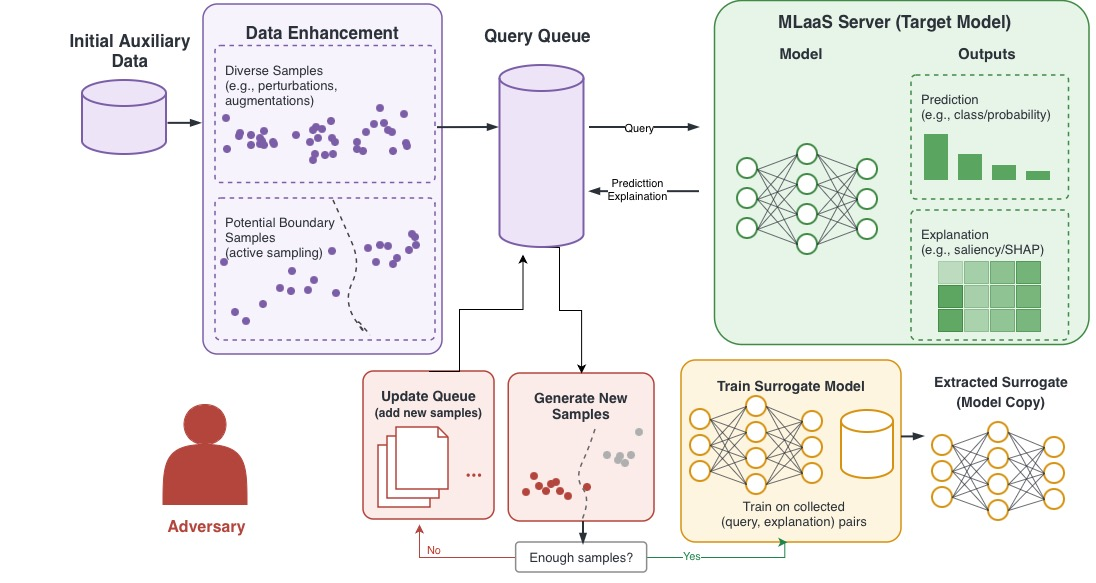
\includegraphics[width=\textwidth]{figures/extraction_pipeline-Page-2.jpg}
\caption{Explanation-guided model extraction pipeline. The adversary enhances a small auxiliary
seed set with \emph{diverse} and \emph{boundary} samples, pushes candidates through a query queue to
the explanation-augmented MLaaS API---receiving a prediction and a post-hoc explanation for each---
uses those explanations to generate new queries, and trains a surrogate on the collected
(query, prediction) pairs until the budget is spent. The data-enhancement stage (diverse generation
and boundary search, \S\ref{subsec:diverse}--\ref{subsec:boundary}) is what we add to the base
attack; the explanation channels it consumes are the subject of our analysis
(\S\ref{sec:analysis}).}
\label{fig:pipeline}
\end{figure*}

Figure~\ref{fig:pipeline} sketches the pipeline.
Autolycus expands a small per-class seed set by local $\pm\varepsilon$ perturbation,
which leaves two systematic gaps that we target directly. First, the surrogate and
target disagree most sharply \emph{at the decision boundary}: concentrating labelled
queries there gives the surrogate a much sharper estimate of the target's decision
surface than the same budget spent in class interiors. Second---and less obvious---we
observe that many surrogate--target disagreements occur on inputs the target classifies
with \emph{high} confidence, i.e.\ confident interior errors rather than boundary
ambiguity. These are \emph{coverage} failures: when the per-class seed set does not
represent the full data distribution, purely local traversal never reaches some regions
of the target, so the surrogate is left confidently wrong there. Diverse query
generation is designed to reach exactly those unvisited regions. Both mechanisms are
consistent with prior extraction results identifying near-boundary and diverse queries
as the two most informative query types~\cite{pal2020activethief}; our aim is not to
rediscover this, but to show \emph{which explanation channel} lets an attacker realise
each cheaply.

We instantiate a single \emph{boundary-directed} extraction attack that adds two components to the
Autolycus traversal~\cite{oksuz2024autolycus}---\emph{boundary search} (Phase~2) and \emph{diverse
query generation} (Phase~1)---and drive it with either explainer
$\mathcal{E} \in \{\textsc{Shap}, \textsc{Lime}\}$. The bin-edge stepping that constitutes
\textsc{Lime}'s threshold channel (Phase~3) is Autolycus's \emph{own} mechanism, retained unchanged
and not something we introduce. The two instantiations share the same three phases and differ
\emph{only} where the decision \emph{threshold} enters the computation (Phase~2 placement and Phase~3
stepping). This is deliberate: it turns the \textsc{Shap}-vs-\textsc{Lime} comparison into a
controlled experiment that isolates the threshold channel (\textbf{H2}), while ablating the
explanation's feature choice isolates the attribution channel (\textbf{H1}). Algorithm~\ref{alg:attack}
summarises the three phases; we describe each below.

\begin{algorithm}[t]
\caption{Boundary-directed explanation-guided extraction, instantiated with explainer
$\mathcal{E}\in\{\textsc{Shap},\textsc{Lime}\}$.}
\label{alg:attack}
\begin{algorithmic}[1]
\Require target API $f$, explainer $\mathcal{E}$, seed set $\mathcal{D}_0$, budget $Q$,
top-$k$, step $\varepsilon$, confidence $\tau$
\Ensure surrogate $\hat{f}$
\State $\mathcal{S} \gets \mathcal{D}_0$;\quad $\mathcal{T} \gets \mathcal{D}_0$
       \Comment{traversal queue $\mathcal{S}$; labelled training set $\mathcal{T}$}
\Statex \textit{// Phase 1: diverse query generation}
\State $\mathcal{C} \gets \textsc{DiverseGen}(\mathcal{S}, \mathcal{E})$
       \Comment{plausibility-filtered or LIME-threshold}
\ForAll{$x \in \mathcal{C}$}
  \If{$\max \hat{p}(x) \ge \tau$} \State $\mathcal{S} \gets \mathcal{S} \cup \{x\}$
  \EndIf
\EndFor
\Statex \textit{// Phase 2: boundary search over cross-class pairs}
\ForAll{cross-class pairs $(a,b)$}
  \State $c \gets$ blend top-$k$ features of $a$ toward $b$
         \Comment{\textsc{Lime}: snap to bin edge; \textsc{Shap}: midpoint}
  \State $(c, M) \gets \textsc{Bisect}(c, b)$ \Comment{8 steps; $M$ = queried midpoints}
  \State $\mathcal{S} \gets \mathcal{S} \cup \{c\}$;\quad
         $\mathcal{T} \gets \mathcal{T} \cup M$ \Comment{recycle midpoints}
\EndFor
\Statex \textit{// Phase 3: explanation-guided traversal}
\While{budget remains \textbf{and} $\mathcal{S} \neq \emptyset$}
  \State $x \gets \textsc{Pop}(\mathcal{S})$;\quad
         $\mathcal{T} \gets \mathcal{T} \cup \{(x, f(x))\}$
  \State select the top-$k$ features of $x$ by $\mathcal{E}$
  \ForAll{selected feature $i$}
     \State $x^{\pm} \gets x$ with coordinate $i$ stepped by $\pm\varepsilon$
            \Comment{\textsc{Lime}: from the bin edge}
     \State add each valid, non-duplicate $x^{\pm}$ to $\mathcal{S}$
  \EndFor
\EndWhile
\State \Return $\hat{f} \gets \textsc{Train}(\mathcal{T})$
\end{algorithmic}
\end{algorithm}

\subsection{Phase 1: Diverse Query Generation}
\label{subsec:diverse-note}
(As noted above, Phase~1 is absent from the base attack on which the channel ablations are run; it
matters for \S\ref{subsec:e4} and \S\ref{subsec:e1} only.)
\label{subsec:diverse}
Autolycus seeds its traversal from a handful of per-class points and expands them by
local perturbation, which tends to under-cover behavioural regions the seeds never
reach. Phase~1 counters this with one of two generators, both returning \emph{unqueried}
candidates that are then queried and kept only if confidently classified
($\max \hat{p}(x) \ge \tau$, $\tau = 0.8$):
\begin{itemize}
  \item \textbf{Plausibility-filtered} (explanation-free): evolutionary crossover and
  mutation of the seed pool, keeping only candidates within a nearest-neighbour distance
  percentile of the real data (a plausibility filter), then selecting by max--min spread.
  This is a purely geometric, explanation-free coverage baseline.
  \item \textbf{LIME-threshold} (explanation-informed): harvest the target's LIME
  bin-edge thresholds \emph{for free} from the already-queried seeds, synthesise
  seed-anchored candidates that \emph{cross} those thresholds into different decision
  cells, plausibility-filter them, and greedily select the candidates covering the most
  distinct $(\text{feature}, \text{threshold}, \text{side})$ configurations. If the
  target surfaces no thresholds (e.g.\ a linear model), it falls back to the geometric
  generator.
\end{itemize}
In its plausibility-filtered form Phase~1 uses no explanation information at all; the
LIME-threshold variant additionally uses the threshold channel. Neither consults the
attribution ranking.

\subsection{Phase 2: Boundary Search}
\label{subsec:boundary}
Phase~2 places training points \emph{on} the decision boundary, where labels are most
informative. For each cross-class pair $(a,b)$ we build a child from $a$ by blending its
top-$k$ features toward $b$, then run an $8$-step bisection between the child and $b$ to
converge onto the boundary between their classes. The explainer governs \emph{how} the
child is placed, and this is precisely where the threshold channel enters:
\begin{itemize}
  \item \textbf{\textsc{Lime}} snaps each continuous top-$k$ feature to its local
  \emph{bin edge} on the side toward $b$---a direct, free estimate of where the boundary
  crosses that coordinate.
  \item \textbf{\textsc{Shap}}, having only magnitudes, places the blend at the
  \emph{midpoint} and must rely on the subsequent bisection to \emph{search} for the
  same boundary location.
\end{itemize}
Every bisection midpoint is queried against the target and therefore carries a label; we
recycle all of them into $\mathcal{T}$ as boundary-concentrated training data (they are
not $\varepsilon$-perturbed further).

\subsection{Phase 3: Explanation-Guided Traversal}
Phase~3 is the Autolycus-style expansion. We pop a sample $x$, query and label it,
explain it with $\mathcal{E}$, select its top-$k$ features (by $|\phi_i|$ for
\textsc{Shap}, by $|w_i|$ for \textsc{Lime}), and emit two children per feature stepped
by $\pm\varepsilon$; valid, non-duplicate children re-enter the queue until the budget is
exhausted or all classes are sufficiently visited. We retain this expansion because it
matters on its own---removing Phase~3 degrades fidelity, most sharply for tree
targets---but the \emph{attribution-based selection} is \emph{not} what drives it:
consistent with \textbf{H1}, replacing the explanation's top-$k$ choice with a random one
leaves fidelity essentially unchanged on our primary (non-tree) targets
(\S\ref{sec:experiments}). What differentiates the two explainers here is, once more, the
threshold channel: \textsc{Lime} steps $\pm\varepsilon$ \emph{from the feature's bin
edge}, so each step crosses the local threshold, whereas \textsc{Shap} steps from the
current value using only the (inert) attribution ranking. Phase~3 therefore contributes
coverage and expansion; its sole explanation-supplied benefit is \textsc{Lime}'s
threshold stepping, not the attribution ranking.

\subsection{Query Accounting}
\label{subsec:accounting}
Following Autolycus, the explanation is bundled with the prediction and \emph{not} charged as a
separate query; only the Phase~2 bisection intermediates consume additional budget. For a fair
comparison we train the surrogate on \emph{every} queried point---Phase-1 candidates, Phase-2
midpoints, and Phase-3 samples---so that $Q$ counts exactly the labelled points available to
$\hat{f}$ and no paid-for query is discarded. Because the Phase-2 overhead can otherwise starve
Phase~3 at small $Q$, a budget-scaling rule caps it to a fixed fraction of $Q$, relaxing at large
budgets. Queries are also deduplicated: a candidate already queried, or already queued, is not
submitted again, since the adversary can cache the response. These are accounting choices inherited
from the baseline, not contributions. Throughout we report fidelity against the query \emph{budget}
$Q$ rather than queries consumed, following the baseline's convention; we return to what this does
and does not favour in \S\ref{subsec:e4}.

Every adversary we compare therefore spends the same counted budget, and \textsc{grid-guided} claims
no advantage from the accounting. It does, however, differ in one deployment-relevant respect: because
it never calls an explanation endpoint, it applies unchanged to services that return predictions
only, which is the majority of deployed prediction APIs and a setting in which an
explanation-guided attack cannot be mounted at all.

% =======================================================================
\section{Analysis: Why Attribution Does Not Suffice}
\label{sec:analysis}
We set out the reasoning behind the two hypotheses of \S\ref{sec:problem}; \S\ref{sec:experiments}
tests them.

\paragraph{Attribution is magnitude, not location (H1).}
An attribution vector $\bm{\phi}(x)$ ranks features by local influence but says nothing about
\emph{where} along a feature the prediction changes. Two attackers handed the same ranking but
stepping to different coordinates place entirely different queries, so the ranking alone cannot
determine query placement. The ranking is moreover a \emph{noisy} guide: although an explainer
selects locally influential features more often than chance, replacing the explanation's top-$k$
choice with a random one leaves surrogate fidelity essentially unchanged (E2,
\S\ref{sec:experiments}). The attribution channel thus carries no signal the attacker can convert
into fidelity beyond a random feature choice.

\paragraph{The threshold is the exploitable channel (H2).}
What an attacker can exploit is a \emph{threshold}: a coordinate at which the prediction changes.
LIME's discretization discloses one for free---each returned $(\text{feature}, \text{bin})$ pair is
a local threshold estimate---so a LIME attacker can place queries directly onto the boundary. SHAP,
carrying only magnitudes, must \emph{search} for that coordinate (e.g.\ by bisection), spending
queries to recover what LIME reveals. This predicts that a threshold-bearing explainer beats a
magnitude-only one on the identical scaffold, and that destroying the threshold---perturbing LIME's
bin edges---collapses the advantage; both are tested in E3 (\S\ref{sec:experiments}). With H1, this
recasts explanation leakage as a matter of decision \emph{thresholds}, not attribution or geometry.

% =======================================================================
\section{Experiments}
\label{sec:experiments}
\subsection{Setup}
\label{subsec:setup}
We evaluate on six public tabular datasets (Table~\ref{tab:datasets}) covering continuous,
categorical, and mixed feature schemas, against five target families: logistic regression (LR), naive
Bayes (NB), $k$-NN, decision tree (DT), and random forest (RF). We scope to tabular data throughout,
following the attack we analyse~\cite{oksuz2024autolycus}. Following the Autolycus convention, the
LIME attacker uses $n{=}1$
seed per class and explores $k{=}3$ top features, and the SHAP attacker uses $n{=}5$ and $k{=}3$.
Query budgets are per dataset (Table~\ref{tab:datasets}); following Autolycus we plot fidelity
against the query \emph{budget} rather than queries consumed (\S\ref{subsec:accounting}).

Compared arms always run on \emph{paired} seed sets (identical draws, identical RNG state), and
surrogate fidelity (Eq.~\ref{eq:sim}) is aggregated by the \emph{mean} over refits. Significance is a
paired Wilcoxon signed-rank test over the $10$ paired observations, with $^{*}p{<}.05$ and
$^{**}p{<}.01$. With $10$ pairs the smallest attainable two-sided $p$-value is $2/2^{10}\approx.002$,
reached only when every pair falls the same way; $^{**}$ therefore marks a near-unanimous effect across
target instantiations rather than an arbitrarily small $p$.

\paragraph{Protocol.} We deviate from the original attack's reporting in two ways, both toward more
conservative estimates. \emph{Surrogate aggregation:} the original trains $R$ surrogate refits per
arm and reports the single one most similar to the target---a quantity measured on the evaluation set,
so the selection is made using the reported metric. We instead report the mean over the $R$ refits,
which is unbiased. ($R$ denotes surrogate refits and is unrelated to the top-$k$ feature budget $k$;
we use $R{=}20$ for DT, $R{=}10$ for RF, and $R{=}1$ otherwise.)
\emph{Target instantiation:} the original varies only the attacker's seed sets against a single fitted
target, so its reported spread reflects seed noise rather than variation across targets. For the
ablations (\S\ref{subsec:e2},~\S\ref{subsec:e3}) we therefore draw $10$ independent train/test splits
and retrain the target on each, pairing all arms within a split, so each observation is an independent
target instantiation. 
We deliberately retain the original single-split protocol for the attack
comparison of \S\ref{subsec:e4}, so that those numbers remain comparable to the published baseline. \TODO{I am not sure if I want to give this as the main result. maybe I'll give our version of comparison in the main theirs in the appendix so put a mark on this sentence, we will decide later}

\begin{table}[t]
\centering
\caption{Datasets. $n$ is the total size; \emph{cont.} counts continuous features (the rest are
categorical, for which \textsc{Lime}'s discretization yields few distinct cut points). Train / eval /
aux follow the $75\!:\!15\!:\!10$ split of the attack we analyse: the target is fit on train, fidelity
is measured on eval, and the adversary's auxiliary sample is drawn from aux. Evaluation-set size sets
the resolution of every per-cell number: one held-out point is $0.06$pp on pendigits but $1.18$pp on
breast, so effects of a few points are resolvable on the former and not on the latter.}
\label{tab:datasets}
\begin{tabular}{lrrrrrrrr}
\toprule
 & $n$ & feat. & cont. & cls. & train & eval & aux & $Q$ \\
\midrule
crop      & $1{,}700$  & 7  & 7  & 17 & $1{,}275$  & $255$   & $170$   & $1000$ \\
adult     & $32{,}561$ & 11 & 3  & 2  & $24{,}420$ & $4{,}884$ & $3{,}257$ & $1000$ \\
breast    & $569$      & 30 & 30 & 2  & $426$      & $85$    & $58$    & $100$  \\
nursery   & $12{,}960$ & 8  & 0  & 3  & $9{,}720$  & $1{,}944$ & $1{,}296$ & $1000$ \\
mushroom  & $8{,}123$  & 21 & 0  & 2  & $6{,}092$  & $1{,}218$ & $813$   & $1000$ \\
pendigits & $10{,}992$ & 16 & 16 & 10 & $8{,}244$  & $1{,}648$ & $1{,}100$ & $500$  \\
\bottomrule
\end{tabular}
\end{table}

\subsection{E4: Attack performance against the published baseline}
\label{subsec:e4}
This experiment uses the \textsc{explanation-matched} configuration of \S\ref{sec:method}, not the
\textsc{grid-guided} attack: both sides read the target's \textsc{Lime} output, so the comparison
isolates query \emph{placement} at equal information access. \S\ref{subsec:ladder} evaluates the
\textsc{grid-guided} attack, which is the one the paper proposes.

Figure~\ref{fig:lime-headline} plots surrogate fidelity against query budget for the
\textsc{explanation-matched} configuration and the Autolycus \textsc{Lime} baseline. At a single
fixed diverse budget it improves fidelity on 18 of 25 target/dataset combinations (10 significant at
$p{<}.05$, against 2 significant regressions), with the most consistent gains on the non-tree targets
that have headroom (LR/NB on crop, nursery, and mushroom).

Establishing that the added phases are worth their budget is what licenses the null results that
follow: a channel that fails to help \emph{this} adversary is not failing for want of a capable
attack.

Part of this margin is an accounting effect worth stating plainly. Autolycus's traversal terminates
when its queue empties, which on several targets happens well before the budget is exhausted; its
curve then flattens because it \emph{cannot} spend the remaining budget, not because additional
queries would not help. Our Phase-1 and Phase-2 components keep generating admissible queries, so they
continue to convert budget into fidelity. Read at equal \emph{budget} the comparison therefore
flatters this configuration, and read at equal \emph{consumed queries} it would flatter Autolycus; we plot
budget because that is the baseline's convention and the quantity a defender actually meters. The
$k{=}3$ control in Appendix~\ref{app:robustness}, where the baseline does spend its full budget,
isolates how much of the margin is saturation rather than better placement.

\begin{figure*}[t]
\centering
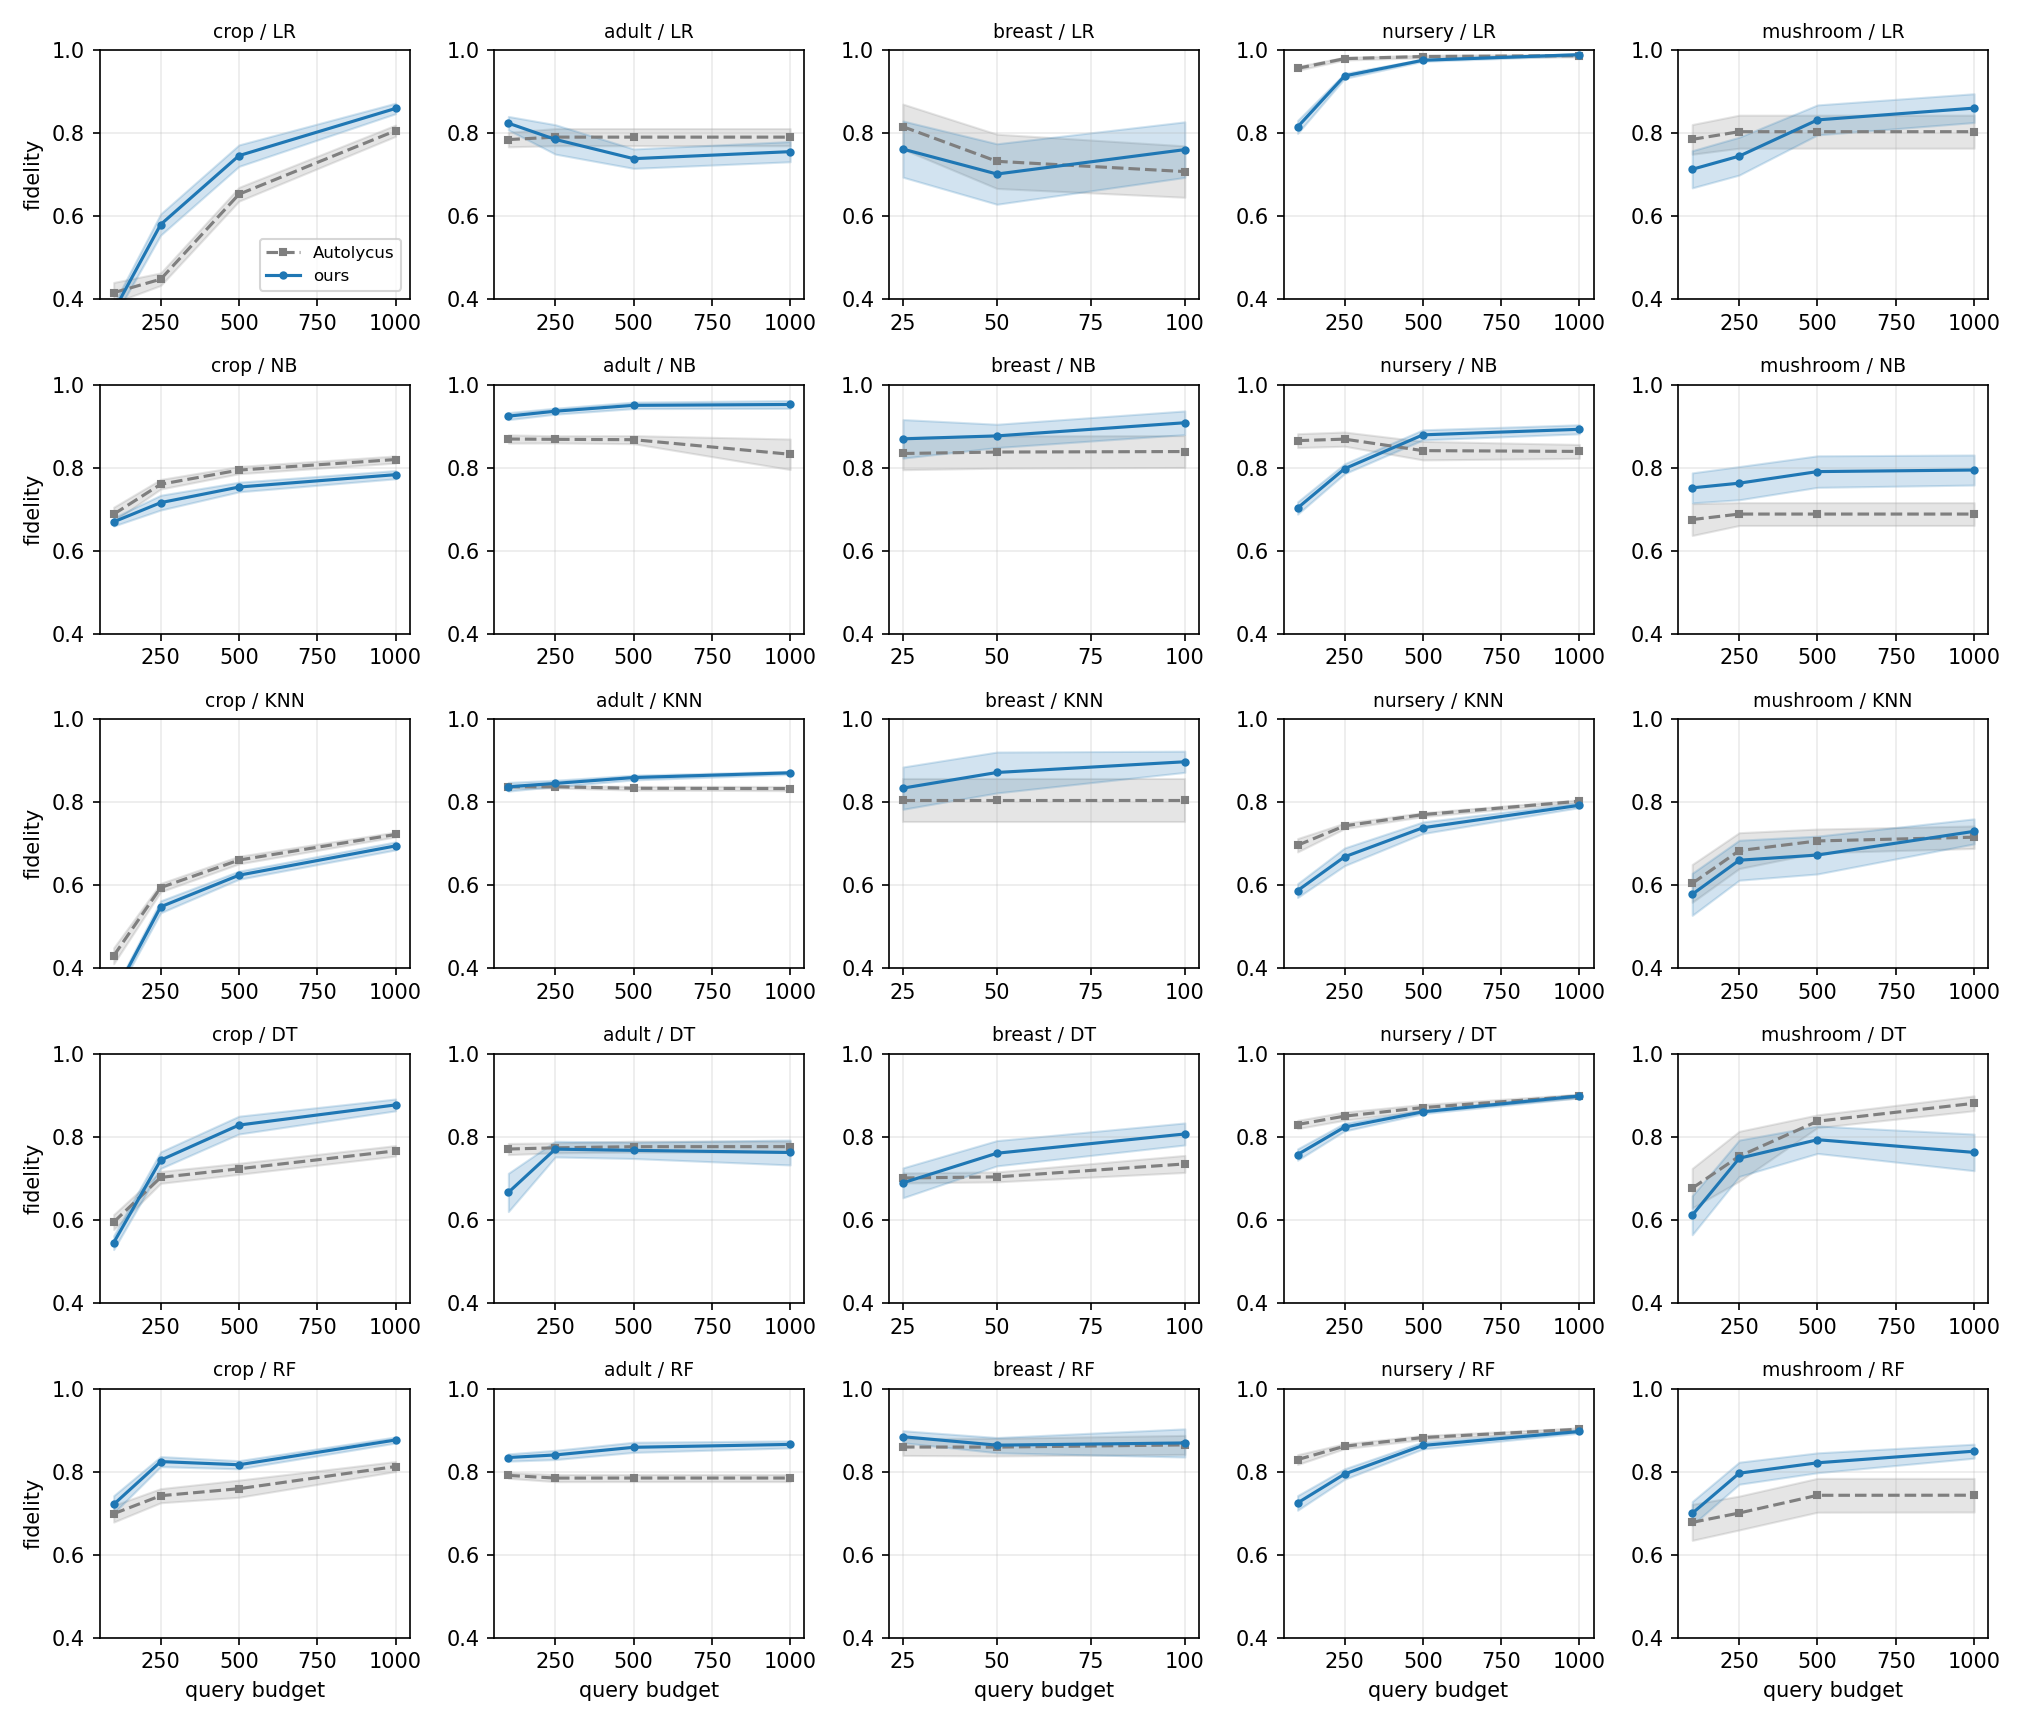
\includegraphics[width=\textwidth]{figures/lime_grid.png}
\caption{E4: surrogate fidelity vs.\ query budget---the \textsc{explanation-matched}
configuration (solid, blue)
vs.\ Autolycus-LIME (dashed, grey), per target (rows) and dataset (columns). Shaded band is the
standard error over the $S{=}10$ seed sets. Ours uses a single fixed diverse budget
(cap${=}15$, not tuned per target); $n{=}1$, $k{=}3$
(breast $Q{\le}100$, others $Q{\le}1000$). All panels share a fixed $y$-axis ($0.4$--$1.0$) for
cross-panel comparability.}
\label{fig:lime-headline}
\end{figure*}

\paragraph{The same attack helps under SHAP.}
Repeating E4 with \textsc{Shap} as the explainer ($n{=}5$, $k{=}3$) gives the same picture: the
\textsc{explanation-matched} configuration improves over Autolycus-\textsc{Shap} on the same non-tree targets (LR/NB/KNN,
largest where the baseline has headroom, e.g.\ nursery and mushroom), while tree targets sit near
their fidelity ceiling and show no gain (Figure~\ref{fig:shap-headline}, Appendix~\ref{app:sweeps}).
That the same boundary-and-diversity machinery helps under \emph{both} explainers---independent of the
particular attribution scores it consumes---is the first indication that the attribution channel is
not what drives the gain (H1); the \textsc{Lime}-specific advantage of a free \emph{threshold} is
isolated separately in E3.

\paragraph{Diverse-budget sensitivity.}
The diverse generation (Phase~1) is regime-dependent: its optimal budget is roughly bimodal,
helping monotonically on high-headroom targets (best at the maximum budget, e.g.\ NB/adult:
$0.61{\to}0.96$ from no-diverse to full) and hurting on near-ceiling or small continuous targets
(best with no diverse). Because the budget is not the contribution, the headline figure fixes it
to a single value (cap${=}15$, the best global choice: $+3.4$pp mean, 18/25 wins) rather than
tuning per target. Fixing it this way costs accuracy on the targets that prefer a different budget,
and we prefer that cost to a per-target tuning that would not be available to a real attacker.

\subsection{E1: Which part of the attack drives the gain?}
\label{subsec:e1}
Our pipeline adds two components to the Autolycus traversal: diverse query generation (Phase~1) and
boundary search (Phase~2). We isolate their contributions with three nested arms on the same seed
sets---Autolycus alone (\texttt{base}), $+$boundary (Phase~2, no diverse), and $+$diverse on top---so
that boundary$\,=\,$($+$boundary)$\,-\,$\texttt{base} and
diverse$\,=\,$full$\,-\,$($+$boundary). Figure~\ref{fig:decomp} reports the result.

The two components contribute about equally on average ($+1.6$ and $+1.8$pp), but \emph{which} one
drives the gain is strongly target-dependent: naive Bayes benefits almost entirely from
\emph{diverse generation} ($+6.4$pp)---a generative model needs distribution coverage---whereas
random forest and logistic regression benefit almost entirely from \emph{boundary search}
($+4.7$, $+2.5$pp), which places labelled points on the decision surface. In every case the gain is
query \emph{placement}, not the attribution ranking: consistent with H1, the components determine
\emph{where} queries land, and (E2) replacing the explanation's feature ranking with a random one
does not systematically change fidelity. One caveat bounds this decomposition: the boundary term as
measured here bundles Phase-2 boundary search with the Phase-3 threshold stepping it inherits from
Autolycus, so it should be read as the combined contribution of both rather than of bisection alone.
\S\ref{subsec:e3} isolates the threshold component directly. Like E4, this decomposition uses the
\textsc{explanation-matched} configuration, so it measures what the two components add \emph{given}
the target's explanation; \S\ref{subsec:ladder} measures what they add without it.

\begin{figure}[t]
\centering
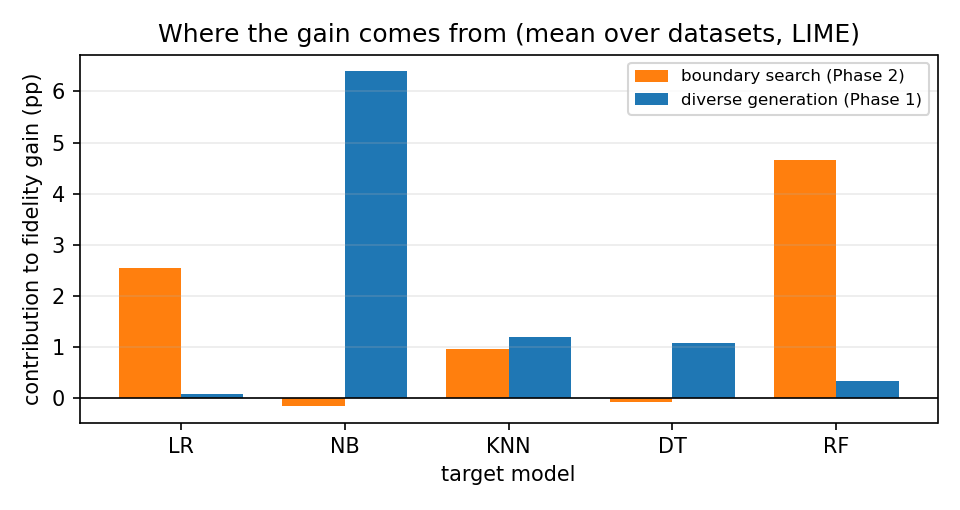
\includegraphics[width=0.9\linewidth]{figures/decomposition.png}
\caption{E1: contribution of each component to the LIME fidelity gain over
Autolycus (percentage points, mean over datasets, top budget). Boundary search dominates for
RF/LR; diverse generation dominates for NB.}
\label{fig:decomp}
\end{figure}

The split is also strongly \emph{dataset}-dependent (Figure~\ref{fig:decomp-perdataset}): diverse
generation carries almost the entire gain on \textsc{adult}/NB ($+34$pp, a generative target starved
of coverage), while boundary search dominates on the tree targets of \textsc{crop} and the linear
targets of \textsc{breast}. Neither component is tied to a particular dataset---both are query
\emph{placement} mechanisms---which is why the aggregate in Figure~\ref{fig:decomp} splits evenly.

\begin{figure*}[t]
\centering
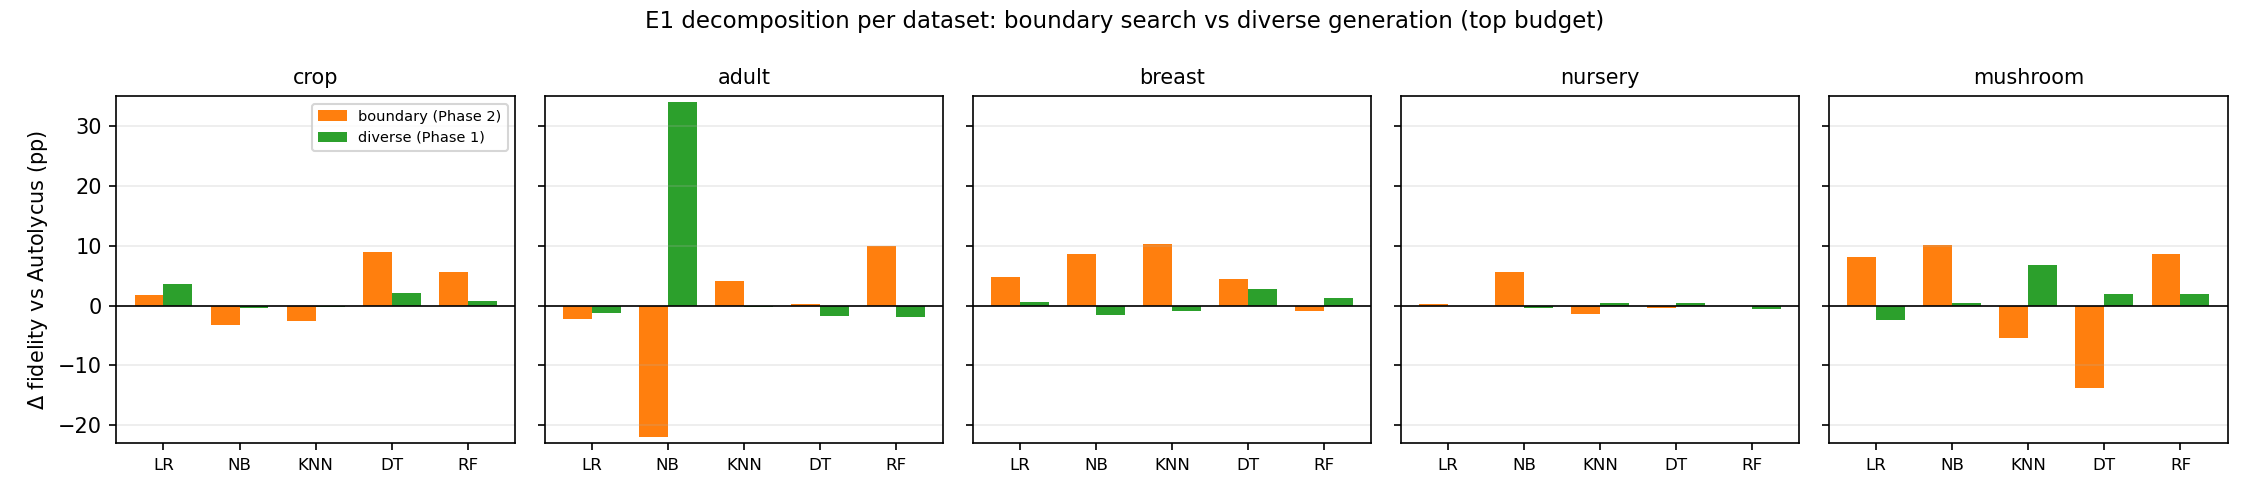
\includegraphics[width=\textwidth]{figures/decomposition_per_dataset.png}
\caption{E1, per dataset: contribution of boundary search (Phase~2, orange) and
diverse generation (Phase~1, green) to the LIME fidelity gain over Autolycus (percentage points, top
budget, mean over $S{=}10$ seed sets), one panel per dataset, grouped by target model. Shared
$y$-axis; the \textsc{adult}/NB diverse bar ($+34$pp) sets the scale.}
\label{fig:decomp-perdataset}
\end{figure*}

\subsection{E2: Is the attribution channel the leak? (H1)}
\label{subsec:e2}
We replace the explanation's top-$k$ feature selection with a random-$k$ choice, holding the rest of
the attack fixed (the \emph{feature} axis of the base-Autolycus $2{\times}2$), and measure the change
in surrogate fidelity. If the attribution ranking carries exploitable signal, random selection should
be worse. Across both explainers the attribution channel is \emph{weak and inconsistent} ($S{=}10$
paired sets):
\begin{itemize}
  \item \textbf{\textsc{Shap}: no net advantage.} On the base Autolycus attack, SHAP-guided selection
  is \emph{no better on average} than random no-explanation traversal (Table~\ref{tab:shap-attr}; mean
  $+0.02$pp over $30$ cells, with $5$ significantly positive and $6$ significantly negative). Where it
  helps it is confined to \emph{tree} targets on datasets with a few dominant features, for which the
  \emph{exact} TreeSHAP pinpoints true splits (\textsc{mushroom} DT $+9.8$, RF $+6.9$;
  \textsc{pendigits} DT $+4.1$pp, all $p{<}.01$). But the same explanation that helps trees on
  \textsc{mushroom} \emph{hurts} logistic regression on that very dataset ($-11.2$pp), and it misleads
  across the board on \textsc{nursery} (LR $-10.2$, NB $-9.1$, KNN $-4.6$pp). The sign of the effect is
  a property of the target, not of the explanation, so an attacker choosing to consult SHAP has no way
  to know whether doing so will help or harm.
  \item \textbf{\textsc{Lime}: no systematic advantage either.} Replacing \textsc{Lime}'s ranking with
  a random choice---holding the threshold available to both arms---changes fidelity by a mean of
  $+0.6$pp and a median of $-0.3$pp, with significant effects in \emph{both} directions
  (Table~\ref{tab:lime-attr}). This is weaker than claiming the channel is inert: individual cells
  show real effects, but their sign is not predictable from the dataset or the target family, so an
  attacker gains nothing it can rely on. The instability is itself informative: individual cells move
  by several points under changes that affect only \emph{which} features the control happens to draw,
  which is what one expects when the quantity being measured is close to zero.
\end{itemize}
So neither explainer's attribution ranking confers a systematic extraction advantage. This is not
merely an absence of significance: the contrast with the \emph{threshold} channel is \emph{directional}.
Over the identical cells, threshold ablation is significantly positive eleven times and significantly
negative \emph{never} (mean $+6.8$pp), whereas attribution is significant in both directions around a
mean of $+0.6$pp (\S\ref{subsec:e3}). One channel has a sign; the other does not.
What \textsc{Lime} supplies is not a useful feature ranking but a decision \emph{threshold}.

\begin{table*}[t]
\centering
\caption{E2 on the \emph{base} Autolycus \textsc{Shap} attack: surrogate fidelity (\%) when features
are selected by \textsc{Shap} importance versus at random, and their difference in percentage points
($n{=}5$, $k{=}3$; $^{*}p{<}.05$, $^{**}p{<}.01$). Multi-split protocol: $10$ independent train/test
splits with the target retrained and the \textsc{Shap} explainer refit on each, arms paired within a
split. Averaged over all $30$ cells the two arms are indistinguishable ($84.5$ vs.\ $84.4$).
Significant effects occur in both directions and their sign tracks the \emph{target} rather than the
explanation: \textsc{Shap} aids trees on \textsc{mushroom} ($+9.8$, $+6.9$) while simultaneously
costing $11.2$ points on logistic regression for the same dataset, and misleads across
\textsc{nursery}.}
\label{tab:shap-attr}
\begin{tabular}{llrrr@{\hskip 2em}llrrr}
\toprule
dataset & model & \textsc{Shap} & random & diff & dataset & model & \textsc{Shap} & random & diff \\
\midrule
crop & LR & $80.0$ & $85.5$ & $-5.5^{*}$  & adult & LR & $85.5$ & $85.5$ & $-0.0$ \\
crop & NB & $74.9$ & $75.9$ & $-1.0$  & adult & NB & $92.0$ & $89.6$ & $+2.5$ \\
crop & KNN & $70.3$ & $69.3$ & $+1.0$  & adult & KNN & $86.3$ & $85.3$ & $+1.0$ \\
crop & DT & $92.3$ & $91.0$ & $+1.3$  & adult & DT & $82.6$ & $81.8$ & $+0.8$ \\
crop & RF & $96.7$ & $96.3$ & $+0.4$  & adult & RF & $91.9$ & $91.3$ & $+0.7$ \\
pendigits & LR & $87.4$ & $86.0$ & $+1.3$  & nursery & LR & $79.5$ & $89.7$ & $-10.2^{**}$ \\
pendigits & NB & $90.2$ & $89.6$ & $+0.5$  & nursery & NB & $54.0$ & $63.1$ & $-9.1^{**}$ \\
pendigits & KNN & $84.2$ & $83.5$ & $+0.7$  & nursery & KNN & $53.9$ & $58.5$ & $-4.6^{**}$ \\
pendigits & DT & $68.5$ & $64.4$ & $+4.1^{**}$  & nursery & DT & $92.2$ & $93.4$ & $-1.1^{*}$ \\
pendigits & RF & $86.1$ & $86.7$ & $-0.6$  & nursery & RF & $92.8$ & $92.1$ & $+0.7^{*}$ \\
breast & LR & $96.9$ & $95.8$ & $+1.2$  & mushroom & LR & $71.5$ & $82.7$ & $-11.2^{**}$ \\
breast & NB & $92.5$ & $91.1$ & $+1.4$  & mushroom & NB & $88.0$ & $84.3$ & $+3.8$ \\
breast & KNN & $88.1$ & $88.5$ & $-0.4$  & mushroom & KNN & $83.6$ & $80.0$ & $+3.6^{*}$ \\
breast & DT & $90.1$ & $87.8$ & $+2.3$  & mushroom & DT & $93.2$ & $83.4$ & $+9.8^{**}$ \\
breast & RF & $93.4$ & $93.2$ & $+0.3$  & mushroom & RF & $95.3$ & $88.3$ & $+6.9^{**}$ \\
\midrule
\multicolumn{2}{l}{\emph{mean, all 30 cells}} & $84.5$ & $84.4$ & $+0.0$ & & & & & \\
\bottomrule
\end{tabular}
\end{table*}

\begin{table}[t]
\centering
\caption{E2 on the \emph{base} Autolycus \textsc{Lime} attack: fidelity gain (percentage points) from
selecting the top-$k$ features by \textsc{Lime}'s ranking rather than at random, with the bin edge
available to both arms ($n{=}1$, $k{=}3$; $^{*}p{<}.05$, $^{**}p{<}.01$). Multi-split protocol: $10$
independent train/test splits with the target retrained on each, arms paired within a split. Because
\textsc{Lime} fits a \emph{sparse} local model and does not score every feature, the random arm
recovers the missing bin edges from the explainer's own discretizer, so the two arms differ only in
\emph{which} features are perturbed and not in whether a threshold is available. $^{\dag}$ marks cells
where more than four of the ten splits produced identical fidelity in both arms, leaving too few
non-tied pairs for a meaningful test. Effects are small and inconsistent in sign---compare the
\emph{threshold} ablation on the identical cells (Table~\ref{tab:lime-threshold}).}
\label{tab:lime-attr}
\begin{tabular}{lrrrrrr}
\toprule
 & crop & pendigits & breast & adult & nursery & mushroom \\
\midrule
LR  & $-3.8^{*}$  & $-0.8$ & $+6.0$      & $-4.5$        & $-0.2$      & \\
NB  & $+6.8^{**}$ & $-1.9$ & $+5.2$      & $-1.8^{\dag}$ & $-6.0$      & \\
KNN & $+4.4$      & $-0.1$ & $+4.0^{\dag}$ & $-0.3$      & $+5.7^{**}$ & \\
DT  & $-2.2$      & $-4.4$ & $-2.7$      & $-6.0$        & $+1.5$      & \\
\bottomrule
\end{tabular}
\end{table}

\subsection{E3: Is the threshold (bin edge) the leak? (H2)}
\label{subsec:e3}
We now isolate the \emph{threshold} axis of the same base-Autolycus $2{\times}2$: with the feature
choice fixed to \textsc{Lime}'s ranking, we perturb from the bin edge \textsc{Lime} exposes (default)
versus from the sample's current value (no-threshold), everything else identical. Because the base
attack already snaps to the bin edge and has \emph{no} boundary search to mask the effect, this is
the cleanest possible test of H2.

\begin{table}[t]
\centering
\caption{E3 on the \emph{base} Autolycus \textsc{Lime} attack: fidelity gain (percentage points) from
perturbing at the exposed \emph{bin edge} vs.\ the current value, features held to \textsc{Lime}'s
ranking ($n{=}1$, $k{=}3$; $^{*}p{<}.05$, $^{**}p{<}.01$). Same protocol, cells, and layout as
Table~\ref{tab:lime-attr}, so the two channels are directly comparable. Positive $=$ the threshold
helps. Effects are large and significant on the well-measured continuous datasets (crop, pendigits)
and are directionally consistent: no cell is significantly negative. \textsc{wine} and
\textsc{breast} are reported for completeness but their evaluation sets are small ($27$ and $85$
samples, i.e.\ $3.70$ and $1.18$pp per sample), so they cannot resolve effects of this size.}
\label{tab:lime-threshold}
\begin{tabular}{lrrrrrr}
\toprule
 & crop & pendigits & breast & adult & nursery & mushroom \\
\midrule
LR  & $+40.9^{**}$ & $+9.2^{*}$   & $-10.2$     & $-1.8$ & $-0.8$      & $-8.7$ \\
NB  & $+24.9^{**}$ & $+5.1^{**}$  & $+11.2^{*}$ & $+0.0$ & $+5.0^{**}$ & $-0.2$ \\
KNN & $+15.2^{**}$ & $-0.0$       & $-0.2$      & $-0.3$ & $+1.0^{**}$ & $+13.9^{**}$ \\
DT  & $+38.0^{**}$ & $+11.1^{**}$ & $+4.8$      & $+2.6$ & $+0.6$      & $+2.1$ \\
\bottomrule
\end{tabular}
\end{table}

\paragraph{The threshold channel is directionally consistent.} On the two datasets whose evaluation
sets can resolve it, the bin-edge signal produces large, significant gains: crop (agronomy, $+15$ to
$+41$pp) and pendigits (pen-trajectory, $+5$ to $+11$pp), across ten independent target
instantiations. The asymmetry is what matters: over these cells the threshold ablation is
significantly positive eleven times and significantly negative \emph{never}, whereas the attribution
ablation on the identical cells is significant in both directions
(Table~\ref{tab:lime-attr}). This is precisely the signal \emph{absent} from \textsc{Shap}: on
pendigits, \textsc{Lime}'s threshold yields $+5$ to $+11$pp while \textsc{Shap}'s attribution yields
$+0.7$pp (n.s.), because Shapley magnitudes carry no ``where'' information. H2 holds where H1 fails.

\paragraph{Scope---the mechanism predicts where the channel is weak.} The threshold channel is
load-bearing only when \textsc{Lime}'s per-feature bin edge is a meaningful proxy for the decision
boundary \emph{and} the base attack has room to improve. Both conditions bite. Where features are
\emph{categorical}, discretization yields few distinct cut points and the channel is correspondingly
weak and unstable: on \textsc{nursery} the effect is at most a few points against $+15$ to $+41$pp on
crop, and it does not reproduce reliably---the NB cell measures $+5.0$ in one run and $+1.0$ in
another differing only in random seed. We report this rather than a clean null because
\textsc{nursery}'s features are label-encoded ordinals, so quartiles do fall on real level
boundaries; but the channel there is too small to support a claim in either direction. Where the target is \emph{near-ceiling} (breast) there is
no headroom for any channel to exploit. We scope all experiments to tabular data, following the attack
we extend; we therefore make no claim about high-dimensional or non-axis-aligned regimes.

\subsection{E5: Is the threshold privileged to the target?}
\label{subsec:e5}
\S\ref{subsec:e3} establishes that the discretization threshold is the channel that matters. It does
not establish that the threshold is \emph{information the service discloses}. \textsc{Lime}'s default
\texttt{QuartileDiscretizer} places its bin edges at the $25/50/75$ percentiles of the explainer's
background data---a statistic of the data distribution that is independent of the model and of the
labels. If an adversary can estimate those percentiles from data it already holds, the discretization
accelerates extraction without disclosing anything.

We test this directly on \textsc{Lime} itself. Holding the traversal, the seeds, and the RNG fixed, we
vary only the data the discretizer is fit on, across three paired arms: \texttt{nothresh} (no bin
edge), \texttt{tgt} (discretizer fit on the target's $X_{\text{train}}$---what the service exposes),
and \texttt{aux} (discretizer fit on the adversary's own auxiliary data). We report
$\text{thr}_{\text{tgt}}$ and $\text{thr}_{\text{aux}}$, each measured against \texttt{nothresh}, and
the privileged advantage $\text{leak}=\texttt{tgt}-\texttt{aux}$.

\begin{table}[t]
\centering
\caption{E5: the threshold channel is self-computable. Every cell in which the threshold channel
significantly helps the attack ($\text{thr}_{\text{tgt}}>0$, $p{<}.05$), across all five datasets,
ordered by effect size. $\text{thr}_{\text{tgt}}$ is the gain from the target's discretizer and
$\text{thr}_{\text{aux}}$ the gain from one the adversary fits on its own auxiliary sample, both
measured against a no-threshold baseline; $\text{leak}$ is their difference, i.e.\ the advantage
attributable to the target's data. Multi-split, $n{=}1$. \emph{No leak term is significant}, and the
largest is $3.1$pp against threshold effects of up to $39.6$pp. We restrict the table to cells with a
real effect because a leak term is uninformative where there is nothing to reproduce.}
\label{tab:auxdisc}
\begin{tabular}{llrrr}
\toprule
dataset & model & thr$_{\text{tgt}}$ & thr$_{\text{aux}}$ & leak \\
\midrule
crop      & LR  & $+39.6$ & $+41.6$ & $-2.0$ \\
crop      & DT  & $+37.4$ & $+37.4$ & $+0.0$ \\
crop      & NB  & $+25.0$ & $+24.3$ & $+0.6$ \\
crop      & RF  & $+22.7$ & $+22.4$ & $+0.3$ \\
crop      & KNN & $+15.1$ & $+18.2$ & $-3.1$ \\
mushroom  & KNN & $+14.0$ & $+16.5$ & $-2.5$ \\
breast    & NB  & $+11.2$ & $+11.9$ & $-0.7$ \\
pendigits & DT  & $+11.1$ & $+9.0$  & $+2.2$ \\
pendigits & LR  & $+9.2$  & $+9.1$  & $+0.1$ \\
pendigits & NB  & $+5.1$  & $+5.1$  & $-0.0$ \\
nursery   & NB  & $+5.0$  & $+4.7$  & $+0.3$ \\
nursery   & KNN & $+1.0$  & $+1.3$  & $-0.3$ \\
\bottomrule
\end{tabular}
\end{table}

\paragraph{The discretization helps, but it is not a disclosure.} Across all twelve cells in which the
threshold channel is significantly positive---spanning five datasets and every target family---the
adversary's own discretizer reproduces the gain (Table~\ref{tab:auxdisc}): on crop,
$\text{thr}_{\text{aux}}$ reaches $+41.6$pp against $\text{thr}_{\text{tgt}}$'s $+39.6$pp, and
\emph{no} leak term is statistically significant---the differences average $-0.4$pp and span $-3.1$
to $+2.2$pp, against threshold effects of up to $+39.6$pp. The sign is inconsistent, the self-computed
grid being marginally better in seven of the twelve cells, which is what one expects of two estimates
of the same quantity rather than of a degraded substitute.
The result covers continuous (crop, pendigits), near-ceiling (breast), and categorical (nursery)
targets alike; if anything it is cleanest on categorical data, where quantiles over a handful of
ordinal levels are estimable from almost any sample. The threshold channel is therefore a
\emph{self-computable} property of the data distribution rather than privileged information about the
model. This reframes the finding of \S\ref{subsec:e3}: what \textsc{Lime}'s discretization supplies is
a data-adaptive grid of candidate cut points that makes boundary-straddling queries cheap---valuable
to an attacker, but not something the service is uniquely able to reveal.

\paragraph{How much auxiliary data this requires.} Self-computation is bounded by the quality of the
adversary's distributional estimate, and the threat model we inherit permits a range of auxiliary set
sizes~\cite{oksuz2024autolycus}. Fitting the discretizer on the full auxiliary partition (the
``comprehensive'' end of that range) gives the result above. Restricting it to the $n{=}1$-per-class
seed set (the minimal end, and the setting the original evaluation uses) preserves the result on crop,
where all leak terms remain insignificant, but degrades it on pendigits, where ten samples must
estimate quartiles over sixteen wide-range continuous features and one leak term becomes significant
($+3.0$pp, $p{<}.05$). A third variant, re-estimating the bins online from the accumulated query set,
performs \emph{worse} than either: the attack deliberately concentrates queries near decision
boundaries, so its own query history is a biased estimator of the marginal distribution the bins are
meant to summarise. The adversary's advantage thus rests on holding a modestly sized representative
sample---not on anything the explanation uniquely reveals.

\paragraph{Why obfuscating the channel is unlikely to defend it.} Because the channel localises to \textsc{Lime}'s
\texttt{discretize\_continuous} step, disabling or coarsening it is the natural candidate mitigation.
Two caveats prevent us from claiming it as a validated defense. First, E5 argues it would be
\emph{insufficient}: an adversary holding a representative auxiliary sample can reconstruct an
equivalent grid, so withholding the discretization removes a convenience rather than the capability.
Second, preliminary attempts to perturb the bins rather than remove them (more bins, rounded edges)
did not reduce extraction. Measuring what a defender actually gains by withholding or distorting the
discretization, against an adversary that adapts by self-supplying it, is left to future work.

% =======================================================================
\begin{table*}[t]
\centering
\caption{The adversary ladder. Fidelity (\%) for each adversary, then the three contrasts that carry
the argument. All arms share the counted budget $Q$, the auxiliary pool, the per-split seeds and the
evaluation set; ten independent target instantiations per cell, paired Wilcoxon, $^{*}p{<}.05$,
$^{**}p{<}.01$. \textsc{self-grid} and \textsc{grid-guided} issue zero explanation calls.
Generated by \texttt{ssm/\_ladder\_table.py}.}
\label{tab:ladder}
\begin{tabular}{llrrrrrrr}
\toprule
& & \multicolumn{4}{c}{fidelity} & \multicolumn{3}{c}{contrast} \\
\cmidrule(lr){3-6}\cmidrule(lr){7-9}
dataset & model & \textsc{blind} & \textsc{autolycus} & \textsc{self-grid} & \textsc{grid-guided}
& ours$-$\textsc{autolycus} & ours$-$\textsc{self-grid} & \textsc{self-grid}$-$\textsc{autolycus} \\
\midrule
crop       & LR   & $38.9$ & $80.4$ & $82.3$ & $91.6$ & $+11.1^{**}$ & $+9.3^{**}$ & $+1.8$ \\
crop       & NB   & $57.5$ & $80.9$ & $72.7$ & $75.4$ & $-5.5^{*}$ & $+2.8$ & $-8.2^{**}$ \\
crop       & KNN  & $53.6$ & $66.6$ & $61.4$ & $63.1$ & $-3.5$ & $+1.7$ & $-5.3^{*}$ \\
crop       & DT   & $40.0$ & $77.6$ & $77.9$ & $89.9$ & $+12.3^{**}$ & $+12.0^{**}$ & $+0.3$ \\
\addlinespace
pendigits  & LR   & $58.8$ & $63.3$ & $62.7$ & $77.6$ & $+14.3^{**}$ & $+15.0^{**}$ & $-0.6$ \\
pendigits  & NB   & $67.3$ & $71.1$ & $71.9$ & $83.1$ & $+12.0^{**}$ & $+11.2^{**}$ & $+0.9$ \\
pendigits  & KNN  & $62.5$ & $62.5$ & $62.8$ & $64.6$ & $+2.1^{*}$ & $+1.8^{*}$ & $+0.3$ \\
pendigits  & DT   & $34.3$ & $41.5$ & $43.0$ & $46.5$ & $+5.1$ & $+3.6$ & $+1.5$ \\
\addlinespace
breast     & LR   & $68.9$ & $62.6$ & $60.7$ & $78.0$ & $+15.4$ & $+17.3$ & $-1.9$ \\
breast     & NB   & $74.1$ & $86.8$ & $80.7$ & $88.9$ & $+2.1$ & $+8.2$ & $-6.1$ \\
breast     & KNN  & $69.1$ & $71.4$ & $66.2$ & $73.8$ & $+2.4$ & $+7.5$ & $-5.2$ \\
breast     & DT   & $63.8$ & $68.8$ & $72.2$ & $73.4$ & $+4.6$ & $+1.2$ & $+3.4$ \\
\addlinespace
adult      & LR   & $81.6$ & $79.5$ & $85.1$ & $86.4$ & $+6.9$ & $+1.3$ & $+5.6^{**}$ \\
adult      & NB   & $87.8$ & $87.7$ & $89.6$ & $89.9$ & $+2.2$ & $+0.2$ & $+2.0^{**}$ \\
adult      & KNN  & $82.8$ & $83.8$ & $84.2$ & $86.7$ & $+3.0^{*}$ & $+2.5^{*}$ & $+0.4$ \\
adult      & DT   & $64.4$ & $71.0$ & $75.1$ & $71.2$ & $+0.2$ & $-3.9$ & $+4.1$ \\
\addlinespace
nursery    & LR   & $98.1$ & $97.9$ & $98.1$ & $97.9$ & $+0.0$ & $-0.2$ & $+0.2$ \\
nursery    & NB   & $84.0$ & $84.1$ & $90.4$ & $80.9$ & $-3.2$ & $-9.5^{**}$ & $+6.3^{**}$ \\
nursery    & KNN  & $69.0$ & $81.5$ & $76.5$ & $71.0$ & $-10.5^{**}$ & $-5.5^{**}$ & $-5.0^{**}$ \\
nursery    & DT   & $87.1$ & $90.5$ & $88.4$ & $88.7$ & $-1.8^{*}$ & $+0.3$ & $-2.0$ \\
\addlinespace
mushroom   & LR   & $85.3$ & $83.6$ & $82.2$ & $80.8$ & $-2.8$ & $-1.4$ & $-1.4$ \\
mushroom   & NB   & $71.3$ & $65.6$ & $76.8$ & $79.7$ & $+14.0^{*}$ & $+2.9$ & $+11.1$ \\
mushroom   & KNN  & $65.5$ & $77.6$ & $72.6$ & $70.4$ & $-7.2$ & $-2.1$ & $-5.1^{*}$ \\
mushroom   & DT   & $72.3$ & $83.7$ & $78.6$ & $77.3$ & $-6.5^{*}$ & $-1.3$ & $-5.2$ \\
\midrule
\multicolumn{2}{l}{\emph{mean}} & $68.3$ & $75.8$ & $75.5$ & $78.6$ & $+2.8$ & $+3.1$ & $-0.3$ \\
\bottomrule
\end{tabular}
\end{table*}

\subsection{E6: What does the adversary actually need?}
\label{subsec:ladder}
E2 and E5 each remove one channel from the base attack. Composing them, and adding back the query
synthesis of \S\ref{sec:method}, yields the question this paper exists to answer: what does an
extraction adversary actually need, and how much of it does the service supply? We answer it with a
\emph{ladder} of four adversaries that differ only in what they are given. All four run the same
framework, the same counted budget, the same auxiliary pool, the same per-split seeds, the same
surrogate family and the same evaluation set:

\begin{itemize}
  \item \textsc{blind}: base traversal, random features, no grid. The floor.
  \item \textsc{autolycus}: base traversal with the target's explanation---its feature ranking
  \emph{and} its bin edges. The published attack.
  \item \textsc{self-grid}: base traversal, random features, bin edges from a discretizer the
  adversary fits on its own auxiliary sample. No explanation call is made.
  \item \textsc{grid-guided} (ours): \textsc{self-grid} plus Phase~1 diverse generation and
  Phase~2 boundary search. No explanation call is made.
\end{itemize}

We report a fifth arm, \textsc{grid-guided}${}+{}$\textsc{lime}, which hands the attack the target's
explanation on top of its own grid, to measure what explanation access is still worth to an adversary
that no longer needs it. Three contrasts carry the argument:
$\textsc{grid-guided}-\textsc{autolycus}$ (does the attack need the explanation endpoint at all?),
$\textsc{grid-guided}-\textsc{self-grid}$ (what do Phases~1--2 add on top of the same grid?), and
$\textsc{self-grid}-\textsc{autolycus}$ (does a self-computed grid substitute for the service's, at
equal phases?).

The two explanation-free arms make \emph{zero} calls to \texttt{explain\_instance}: the bin edges they
consume are read directly from the adversary's own discretizer, which is fit on its auxiliary pool
when the explainer is constructed and never touches the target. This is verified by instrumenting the
explainer, not assumed.


\paragraph{The grid matters; its source does not.} Compare \textsc{blind} against the two
grid-holding base-traversal arms. The grid is the largest single effect in the paper: on crop it moves
fidelity from $38.9$ to $82.3$ (LR) and $40.0$ to $77.9$ (DT), and it is what separates a usable
adversary from a hopeless one. But its \emph{source} does not matter. Across all twenty-four cells
$\textsc{self-grid}-\textsc{autolycus}$ averages $-0.3$pp with significance in both directions
(3 positive, 4 negative), and the balance is the same when the data are split by feature type
($-0.4$pp on the continuous datasets, $-0.1$pp on the categorical ones). An adversary that computes
its own discretization from an auxiliary sample is, to within noise, exactly as well off as one handed
the target's explanation---and here that arm reads \emph{nothing} from the explanation, neither the
ranking nor the edges, so the substitution is complete rather than partial.

\paragraph{What the query-synthesis phases add.} The contrast
$\textsc{grid-guided}-\textsc{self-grid}$ isolates Phases~1--2 given an identical grid. It is
$+3.1$pp over all cells (6 significantly positive, 2 negative), and the aggregate hides a sharp and
mechanically predictable split: on the four datasets with continuous features it is $+5.7$pp with
\emph{six significant gains and no significant losses}, while on the two fully categorical datasets it
is $-2.1$pp. The same split governs the comparison against the published attack:
$\textsc{grid-guided}-\textsc{autolycus}$ is $+5.3$pp (6 significant gains, 1 loss) on continuous data
and $-2.3$pp on categorical data.

The mechanism explains the boundary rather than excusing it. Phases~2 and~3 place queries by snapping
a feature to a bin edge; a purely categorical dataset has no continuous axis to discretize, so there
are no edges to snap to and the two phases degenerate to a random-feature traversal that is strictly
worse than following the explanation. This is the same scope condition that made the threshold channel
flat on adult in \S\ref{subsec:e3}, arriving from the other direction, and it bounds the attack
honestly: \emph{grid-guided extraction is an attack on tabular targets with continuous features}. Where
that condition holds it dominates the explanation-guided baseline while querying no explanation at all;
where it does not, the explanation retains genuine value---most visibly on nursery/KNN, where
\textsc{autolycus} reaches $81.5$ against $71.0$ for \textsc{grid-guided}.

Neither component suffices alone. \textsc{autolycus} already holds a grid and is beaten on continuous
data; \textsc{blind} runs the same traversal without one and is far worse than either. The gain is an
interaction---bisection and diverse generation along grid-snapped coordinates---rather than a property
of the grid or of the phases separately.

\section{Discussion and Limitations}
\label{sec:discussion}
\paragraph{Where the leak lives.} Our decomposition recasts explanation-guided extraction as a
question about \emph{decision thresholds}. The exploitable signal is not the attribution magnitude
(\S\ref{subsec:e2}) nor, as prior framings imply, the boundary \emph{geometry}, but the discretization
threshold \textsc{Lime} publishes for free (\S\ref{subsec:e3}). \textsc{Shap}, which reports magnitude
without a threshold, carries no comparable signal. The practical consequence is asymmetric: an MLaaS
provider can serve \textsc{Shap}-style magnitude attributions at substantially lower extraction risk
than \textsc{Lime}-style discretized explanations.

\paragraph{What kind of information the threshold is.} \textsc{Lime}'s default bin edges are the
$25/50/75$ percentiles of the explainer's background data---a property of the data distribution, not
of the model or its labels. The channel we identify is therefore best read as a data-adaptive grid of
candidate cut points that lets the attacker place boundary-straddling queries cheaply, rather than as
a disclosure of the model's own decision surface. Whether an adversary can substitute a grid estimated
from its own auxiliary data---in which case the discretization is a convenience rather than a
disclosure---is the natural next question, and we regard it as open.

\paragraph{Scope and limitations.} The threshold channel is not universal, and we do not claim it is.
It is load-bearing only for continuous tabular targets with fidelity headroom (crop, pendigits); on
categorical features it is an order of magnitude weaker, since discretizing a few ordinal levels
yields few usable cut points, and on near-ceiling targets it is absent because the attack is already
saturated. We scope to tabular data throughout, following the attack we extend, and make no
claim about high-dimensional or non-axis-aligned domains.

The attack inherits exactly this boundary, and it is the sharpest limitation we report.
\textsc{Grid-guided} extraction places queries by snapping features to bin edges, so it requires
continuous features to snap to. On the four datasets that have them it beats the explanation-guided
baseline by $5.3$pp with six significant gains and one loss; on the two purely categorical datasets it
loses by $2.3$pp, and there the target's explanation retains genuine value
(\S\ref{subsec:ladder}). We report that boundary rather than restricting the evaluation to the
datasets where the attack wins. The consequence for a defender is not symmetric with the consequence
for an attacker: the substitutability result of \S\ref{subsec:e5} holds on \emph{all} six datasets,
so withholding explanations does not protect a categorical-feature service either---it merely leaves
our particular attack without an edge to exploit.

Two measurement caveats bound what our per-cell numbers can support. First, \emph{evaluation-set size}
governs resolution: fidelity on \textsc{wine} is measured over $27$ held-out points ($3.70$pp per
sample) and on \textsc{breast} over $85$ ($1.18$pp), against $255$ for crop and $1648$ for pendigits.
Effects on the two small sets are not resolvable at the magnitudes of interest, and we therefore rest
no claim on them---a caution that applies equally to prior work reporting per-cell fidelity on small
splits. Second, our threshold ablation does not run \textsc{Lime}$\times$RF at full budget (traversal
cost), so the ensemble case is not covered. Finally, the crossing-rate objective in Phase~1 is a proxy
for decision-cell coverage.

\section{Conclusion}
Decomposing an explanation-guided extraction attack into an attribution channel and a threshold channel
shows that the attribution ranking---in both \textsc{Lime} and \textsc{Shap}---confers no systematic
advantage, being centred on zero and inconsistent in sign. The one channel that reliably helps is the
decision threshold \textsc{Lime}'s discretization exposes, worth up to $41$ fidelity points and
directionally consistent. That threshold, however, is a quantile of the data distribution rather than a
property of the model, and an adversary holding a representative auxiliary sample reconstructs an
equivalent grid with no measurable loss. What an explanation contributes to extraction is therefore
query-placement convenience, not disclosure---which also means that obfuscating the channel is unlikely
to defend it. Characterising what a defender can actually withhold from an adaptive adversary remains
open.

% ==== Back matter (outside the 12-page main body) ====
\appendix

\section{Query-budget sweeps}
\label{app:sweeps}
\label{app:robustness}
This appendix collects the fidelity-versus-budget sweeps that compare our pipeline against Autolycus.
All of them use the \textsc{explanation-matched} configuration of \S\ref{sec:method}, so both sides
read the target's explanation; the \textsc{grid-guided} attack is evaluated in \S\ref{subsec:ladder}.

Figure~\ref{fig:shap-headline} is the \textsc{Shap} companion to Figure~\ref{fig:lime-headline},
discussed in \S\ref{subsec:e4}. The remaining two vary \textsc{Lime}'s seed count and feature budget:
the main experiments use $k{=}3$, $n{=}1$ (the Autolycus setting), and we report here two alternative
settings under the identical protocol and fixed diverse budget of the main text.

\begin{figure*}[t]
\centering
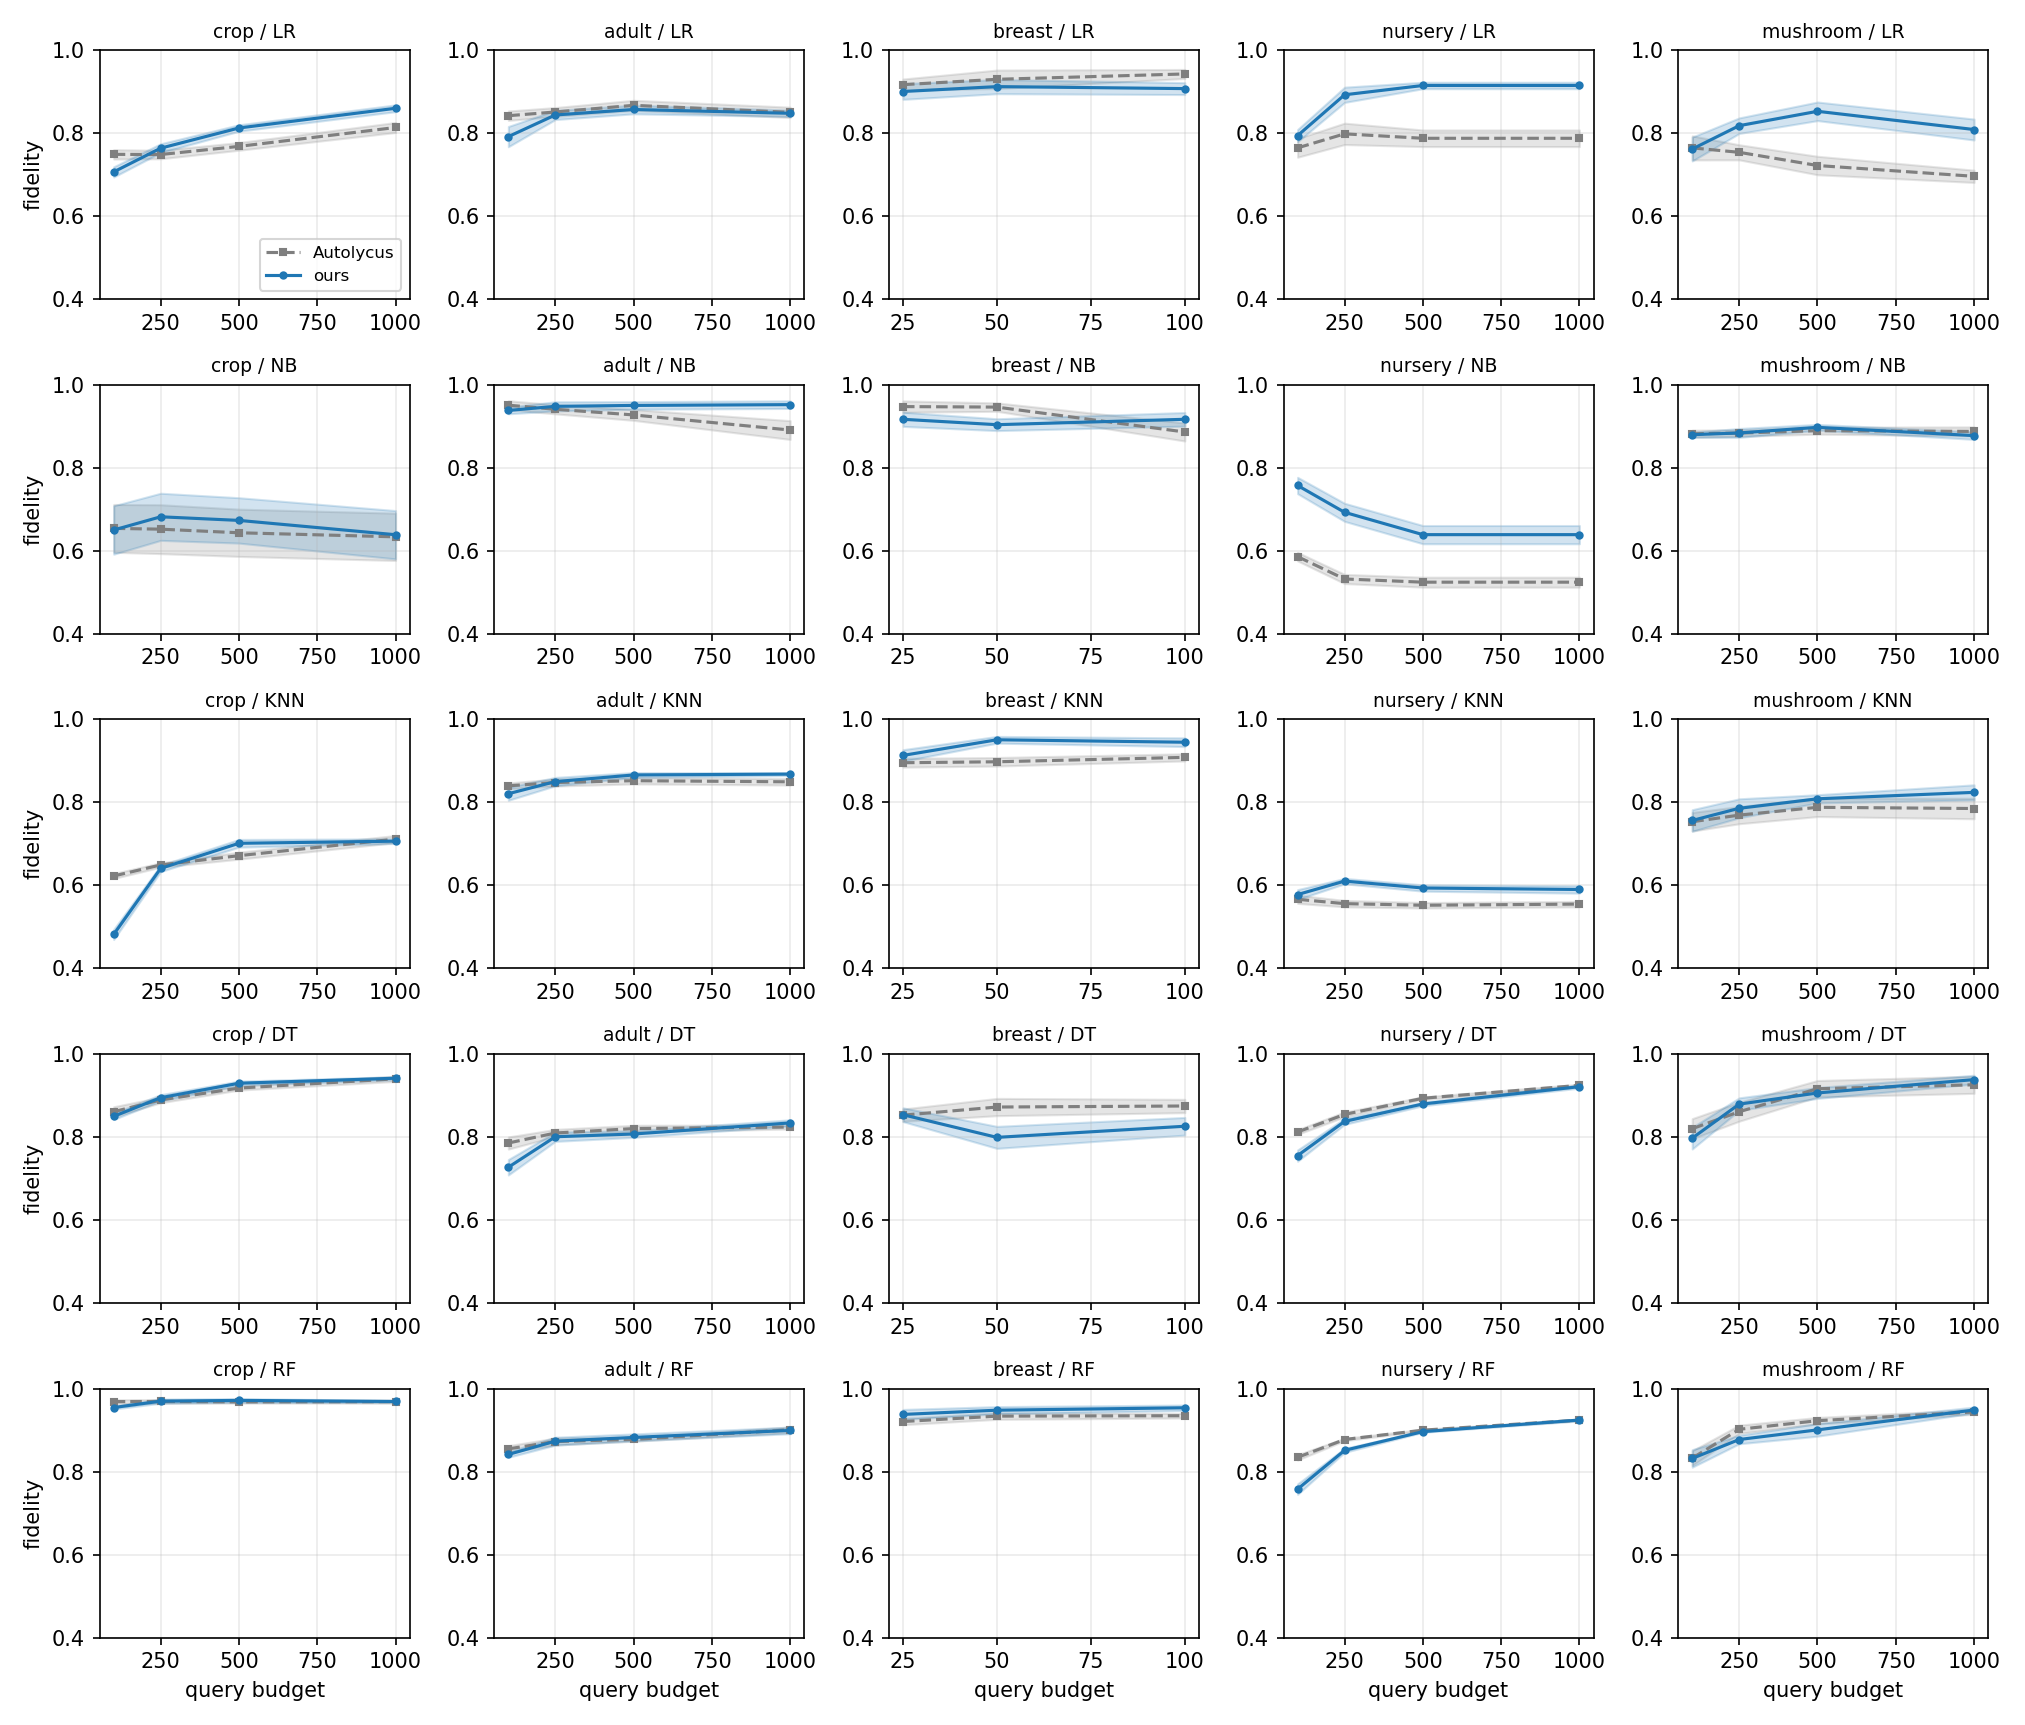
\includegraphics[width=\textwidth]{figures/shap_grid.png}
\caption{SHAP companion to E4: surrogate fidelity vs.\ query budget---the \textsc{explanation-matched}
configuration under \textsc{Shap}
(solid, blue) vs.\ Autolycus-\textsc{Shap} (dashed, grey), per target (rows) and dataset (columns).
Shaded band is the standard error over the $S{=}10$ seed sets; $n{=}5$, $k{=}3$. All panels share a
fixed $y$-axis ($0.4$--$1.0$) for cross-panel comparability.}
\label{fig:shap-headline}
\end{figure*}

Figure~\ref{fig:grid-n3k1} ($k{=}1$, $n{=}3$) shows the largest apparent margin over Autolycus, but
this is an artefact of \emph{base saturation}: at $k{=}1$ Autolycus's traversal exhausts its queue
and cannot spend the budget---its curves go flat---while our diverse generation keeps placing
queries. Figure~\ref{fig:grid-n3k3} ($k{=}3$, $n{=}3$) is the fair control: more seeds, but
Autolycus also uses the full budget. There the mean margin is \emph{smaller} than at $n{=}1$
($+1.9$ vs $+3.4$pp), because additional seeds help Autolycus as much as us. We therefore keep
$k{=}3$, $n{=}1$ as the headline; the larger $k{=}1$ margin reflects Autolycus's budget
under-utilisation, not a seed advantage of our pipeline.

\begin{figure*}[t]
\centering
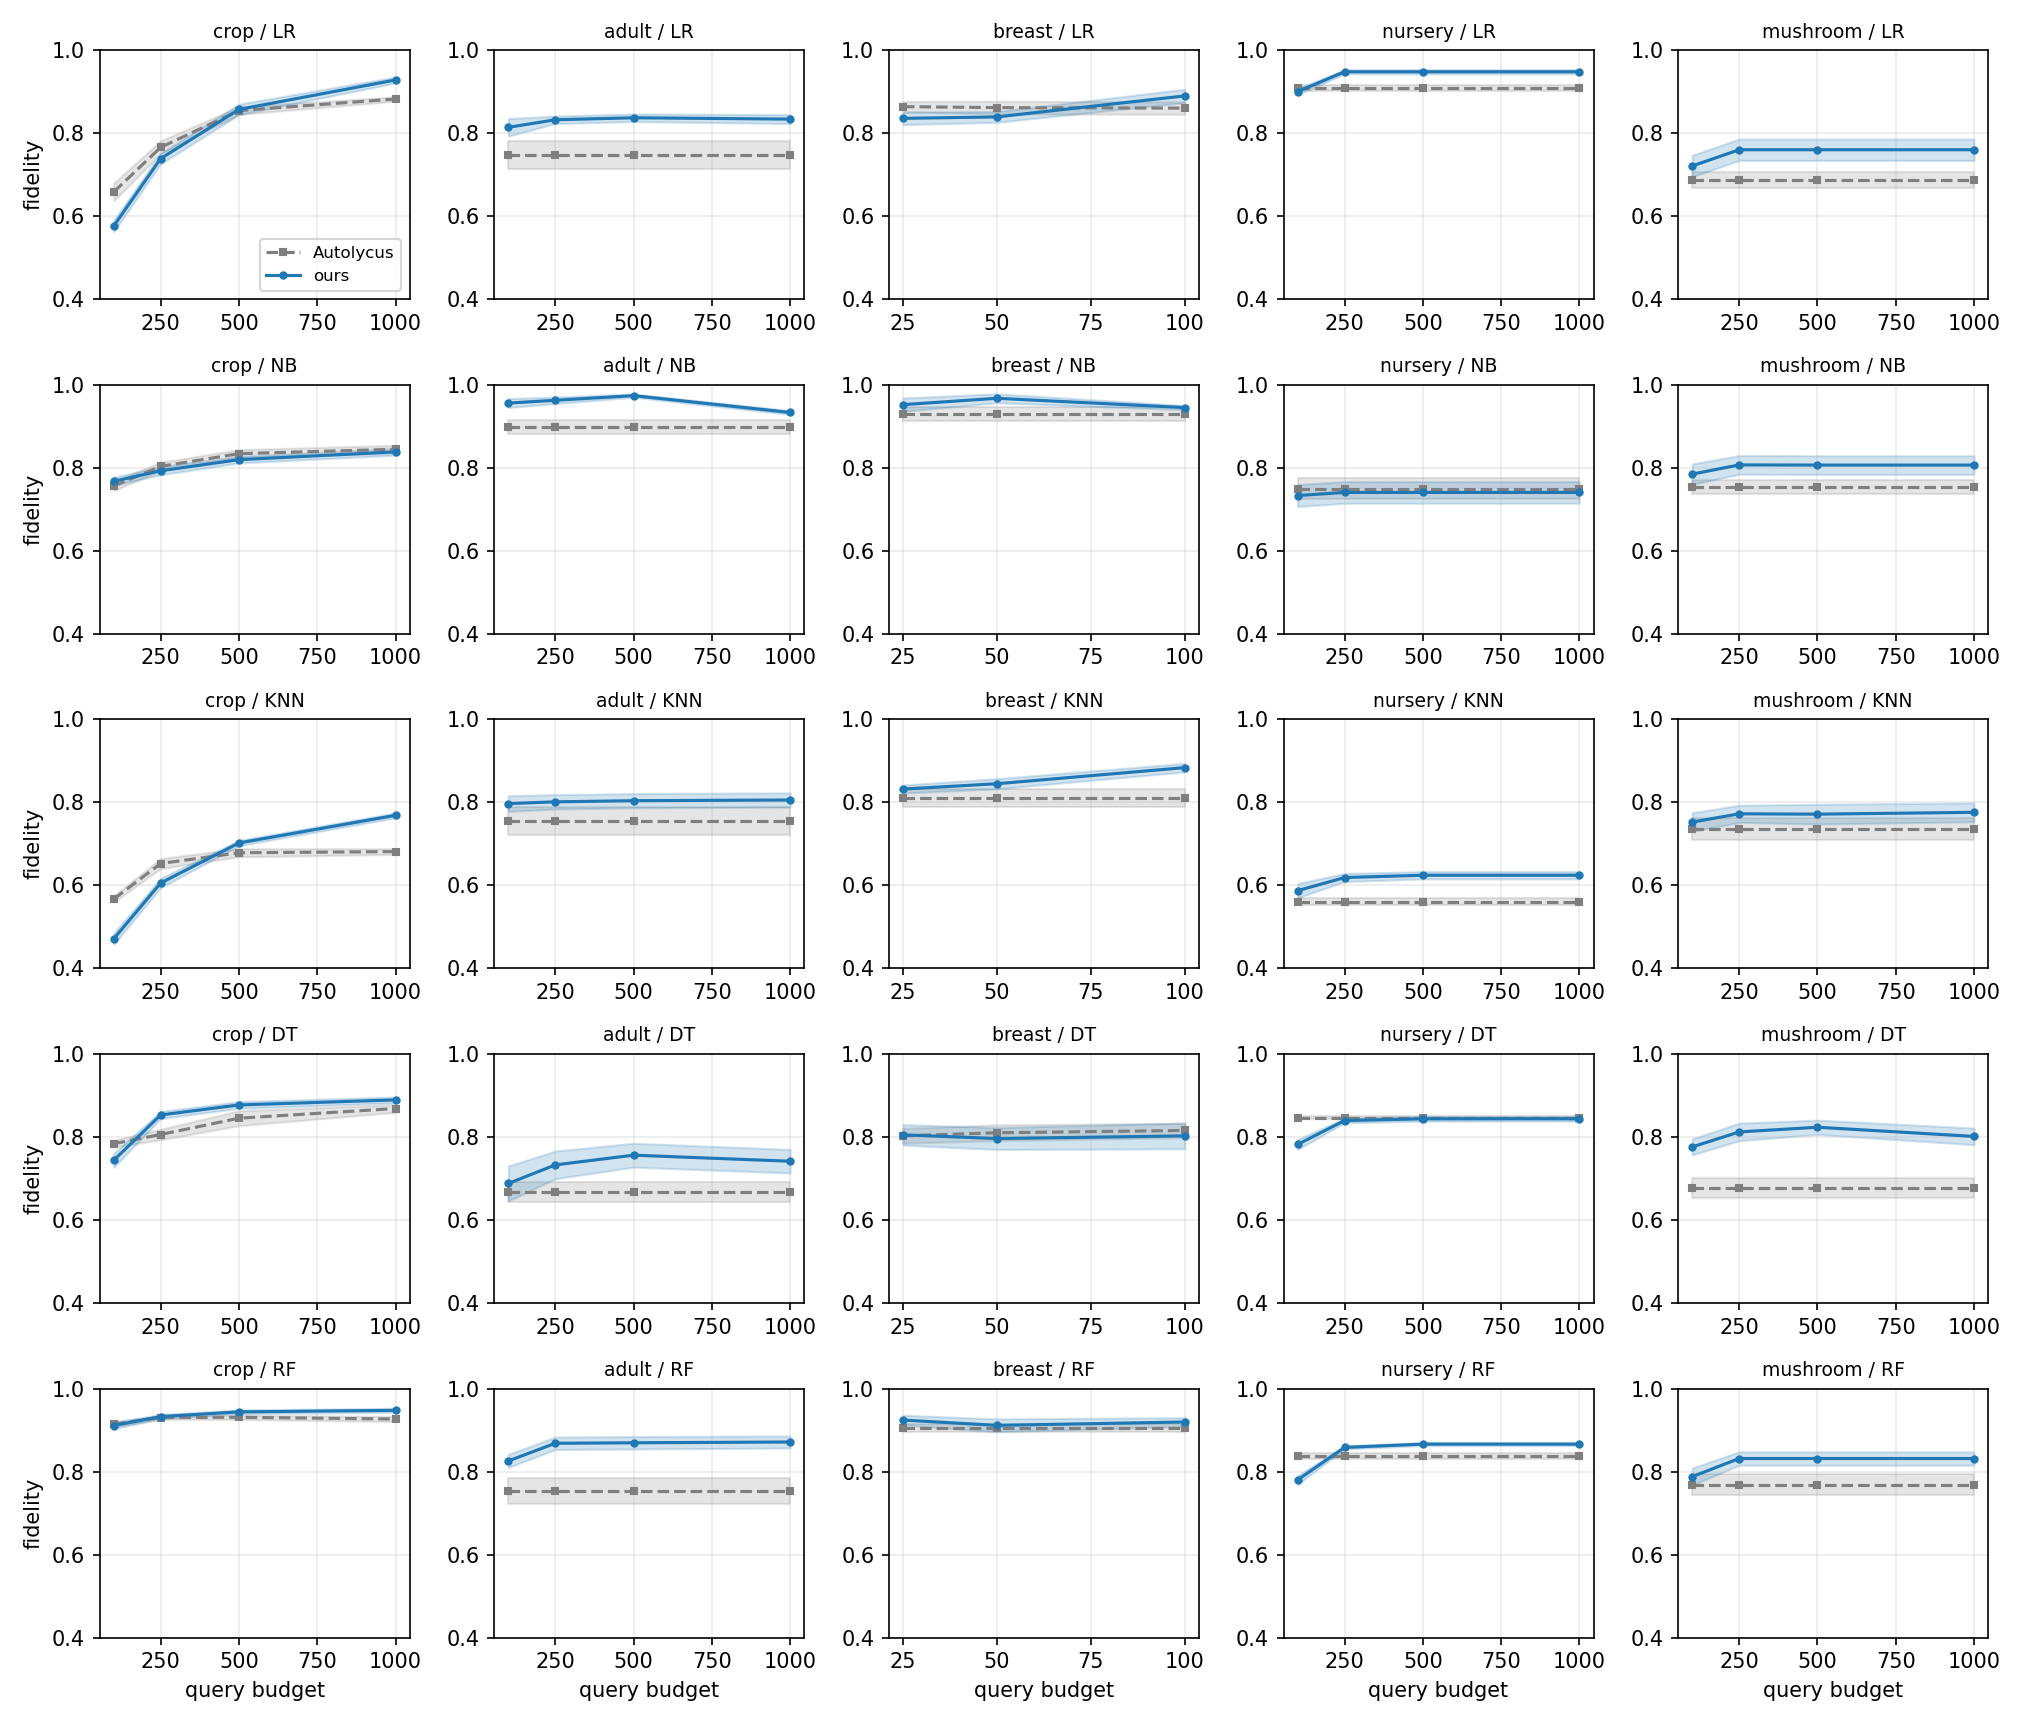
\includegraphics[width=\textwidth]{figures/lime_grid_n3_k1.png}
\caption{LIME at $k{=}1$, $n{=}3$ (secondary). Fidelity vs.\ query budget, ours (blue, solid) vs.\
Autolycus (grey, dashed); band $=$ standard error over 10 sets. Autolycus's curves flatten
early---its traversal saturates at $k{=}1$. Shared fixed $y$-axis ($0.4$--$1.0$).}
\label{fig:grid-n3k1}
\end{figure*}

\begin{figure*}[t]
\centering
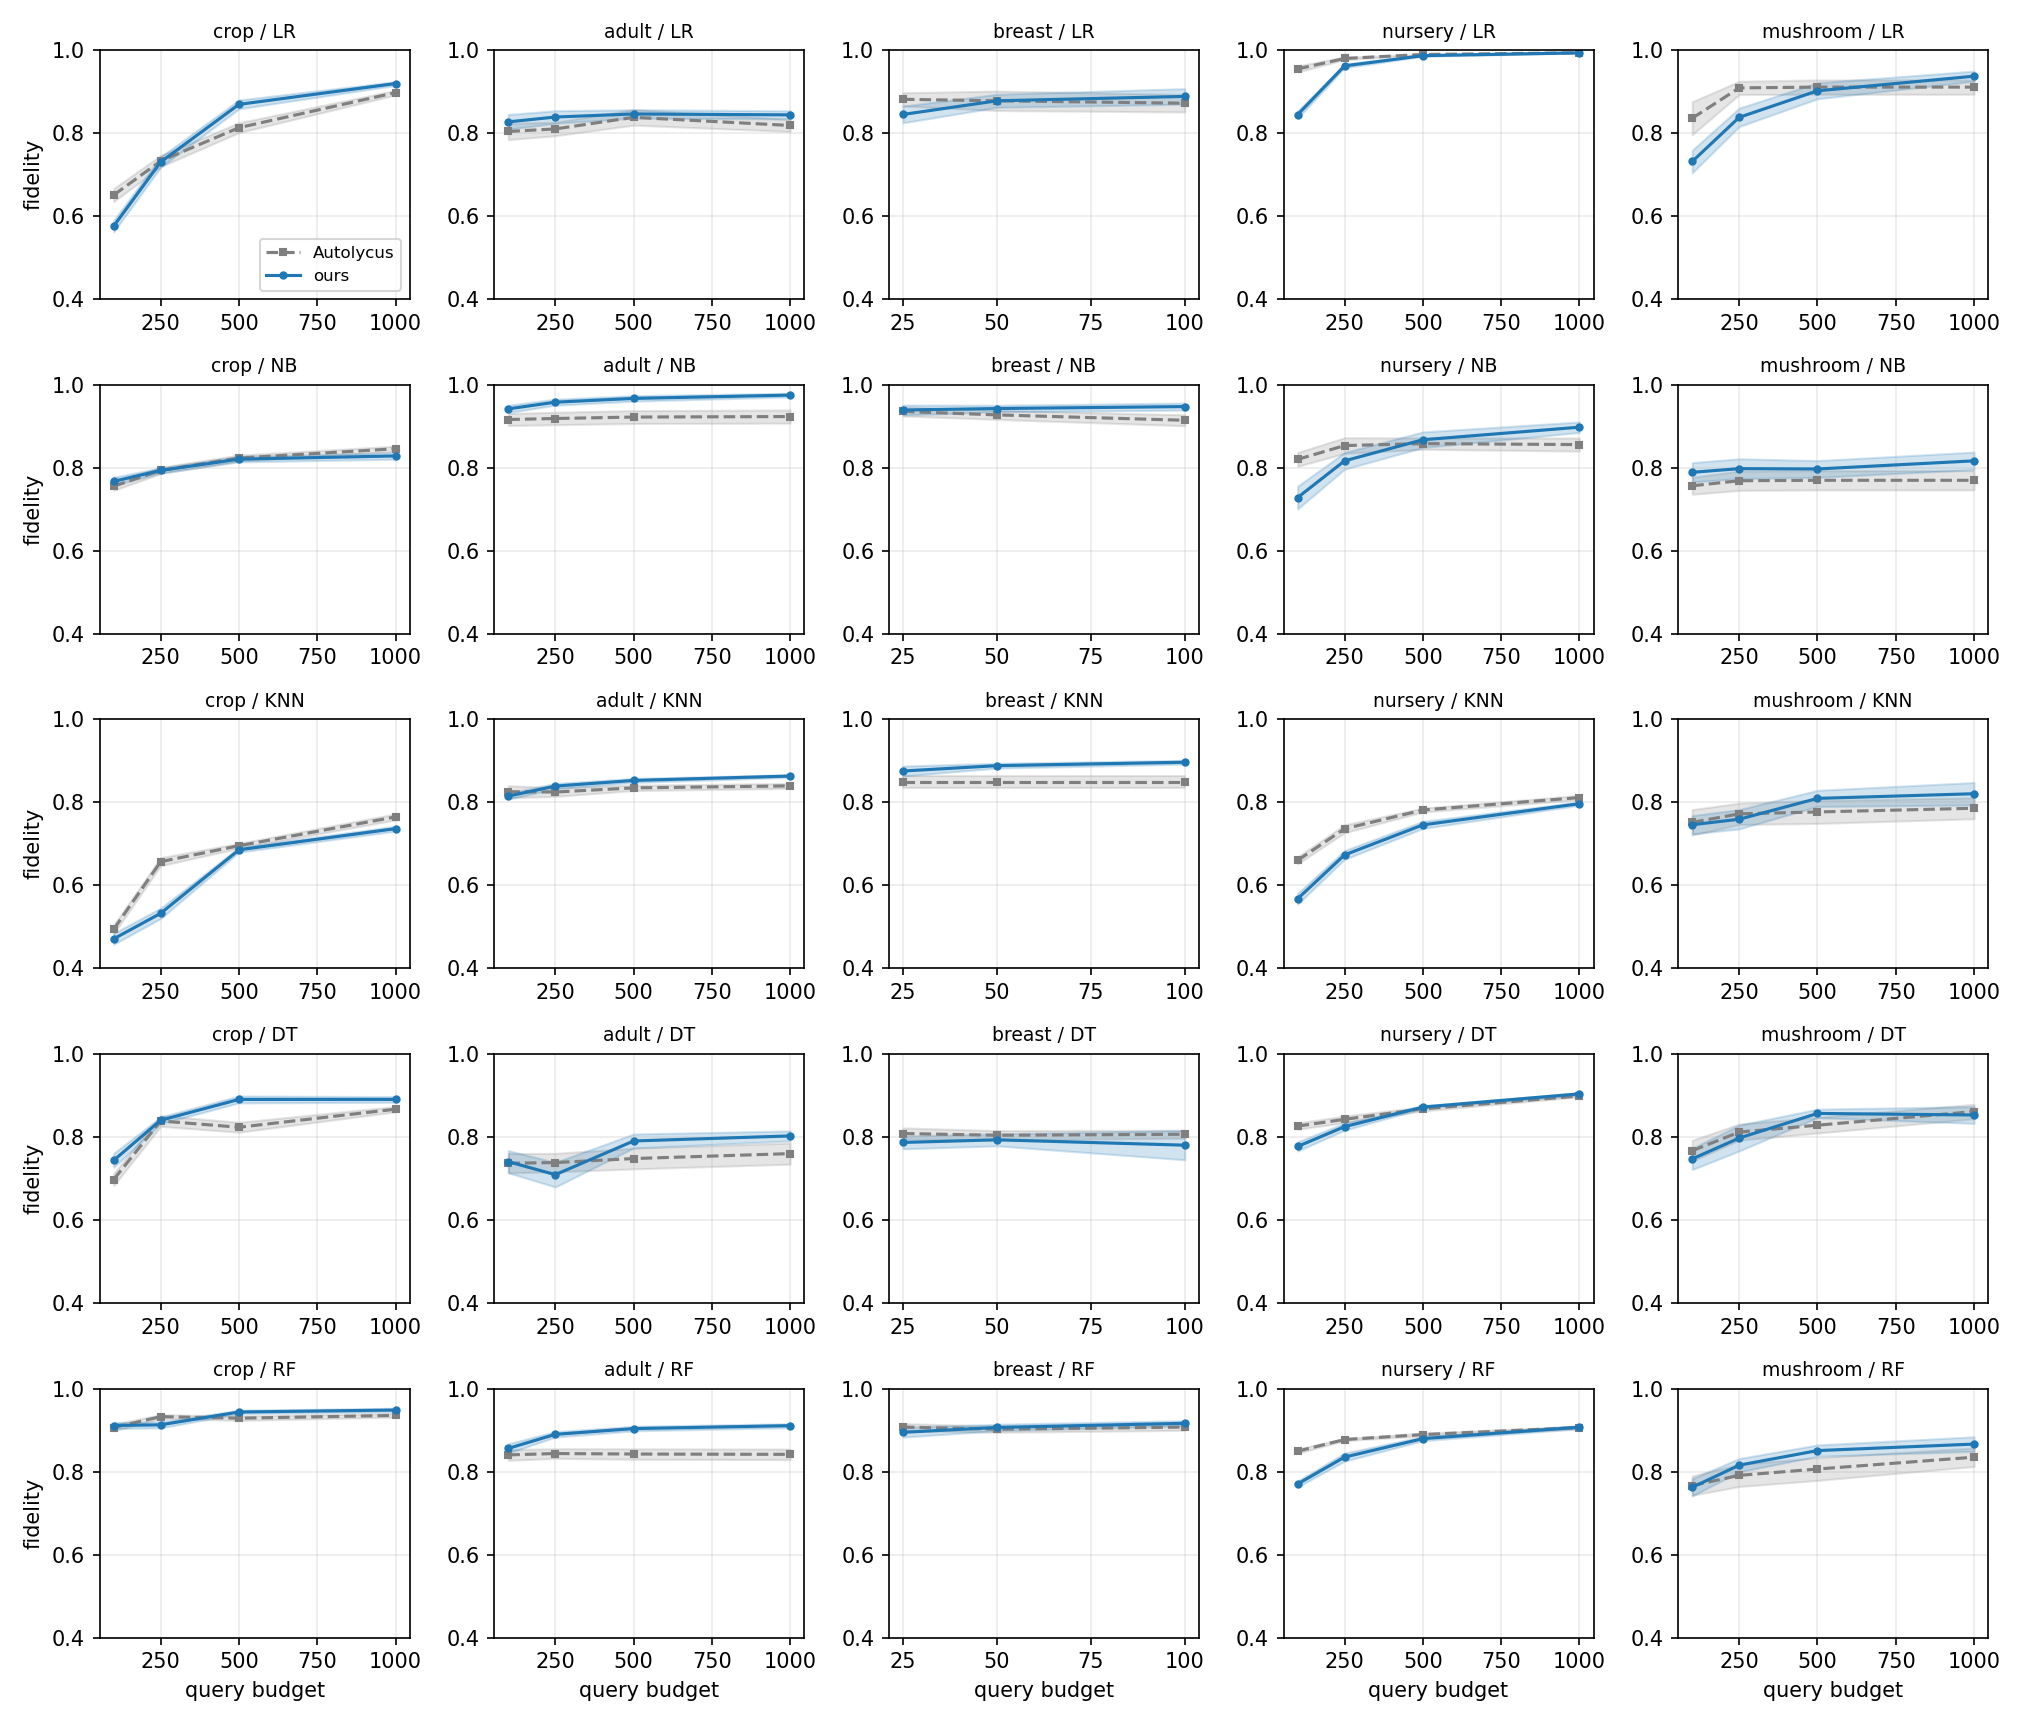
\includegraphics[width=\textwidth]{figures/lime_grid_n3_k3.png}
\caption{LIME at $k{=}3$, $n{=}3$ (fairness control). With $k{=}3$ Autolycus uses the full budget,
and our margin over it is smaller than at $n{=}1$---confirming the larger $k{=}1$ margin is base
saturation, not a seed benefit. Shared fixed $y$-axis ($0.4$--$1.0$).}
\label{fig:grid-n3k3}
\end{figure*}

% Acknowledgements are camera-ready only; omitted under anonymous review.
%\begin{acks}
%\end{acks}

\begin{ethics}
This work studies an \emph{attack}---model extraction guided by post-hoc
explanations---in order to characterise a concrete privacy risk of explainable
machine-learning services. All experiments use publicly available benchmark
datasets and target models that we train ourselves; no proprietary system, personal data,
or live service was queried, and no human subjects were involved. The techniques extend
already-published extraction attacks and are evaluated in a controlled setting, so we
assess the incremental disclosure risk as low. Our findings are, on balance,
risk-\emph{reducing}: we show that the model-specific content of an explanation contributes
little to extraction, and that the component which does contribute is one an adversary can
reconstruct without the service's help. This bounds the incremental risk that publishing an
explanation creates, rather than expanding it. The work was not submitted to an external ethics board, as it involves no
human-subjects or live-system experimentation.
\end{ethics}

\begin{openscience}
We will release our attack implementation and evaluation harness, together with scripts
to reproduce every figure and table, upon acceptance. All datasets used are already public.
% BEFORE SUBMISSION: add an anonymised artifact link (e.g. anonymous.4open.science) here for review.
\end{openscience}

\begin{ai}
AI-based tools were used to assist with drafting and revising the text (improving flow and
correcting phrasing), to help search for related work, and for pre-submission review. The
authors have manually verified, and are responsible for, the accuracy, originality, and
integrity of all content, including every technical claim, experiment, and citation.
\end{ai}

\bibliographystyle{ACM-Reference-Format}
\bibliography{references}

% ==== Appendices (lettered; outside page limit) ====
% \section{...}  % e.g. SHAP4b threshold-densification ablation, if included.

\end{document}
